\chapter{Application of transmission lines}
This chapter deals with the applications of Transmission line at high frequency. In the previous lecture, we dealt with the
analysis of Transmission line i.e. the derivation of transmission line equations, power flow in Transmission Line, voltage and wave characteristics of Transmission Line, the use of graphical tool called a Smith Chart to analyze the Transmission Line.
There are many applications of Transmission Line but at high frequency, many of the reactive elements are replaced by Transmission Line sections. This is the part we shall discuss in this chapter.

\textbf{APPLICATIONS OF TRANSMISSION LINES.}
\begin{enumerate}[(i)]
\item Measurement of Unknown Impedance 
\item Used as Circuit Element
\item StepUp Transformer 
\item Matching Impedance
\end{enumerate}

\section{MEASUREMENT OF UNKNOWN IMPEDANCES}
The measurement of phase is a very difficult task at high frequency, while the amplitude of a signal can easily be measured
in a laboratory. In order to measure complex impedances, the complex voltage and complex current have to be measured. Since the measurement of phase is not that simple, the measurement of complex impedance becomes difficult at high frequency. In transmission line, the temporal phase between the voltage and current gets translated into spatial phase in the form of standing wave pattern.
Which means we can assume that the temporal phase between voltage and current, is gotten by measuring the standing wave pattern on the transmission line. This is the method used for measuring unknown impedance at high frequency, using a special transmission line called \textbf{slotted
transmission line}.
\begin{figure}[h]
\centering
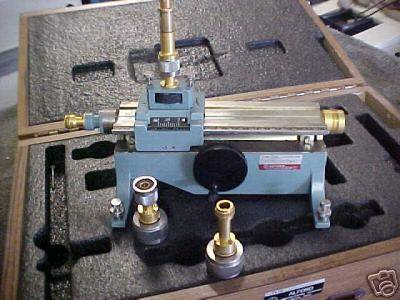
\includegraphics[width=1\linewidth]{./graphics/slottedT}
\caption{Slotted Transmission Line}
\end{figure}

The slotted transmission line consists of a movable probe inserted in a slot in a Transmission Line. It is also used for measuring standing waves, wavelength, minimum and maximum voltage. In the measurement of unknown impedance, it gives us access to the transmission line in real time, to measure the voltage amplitude of the standing wave found on it.

The groove in the slotted transmission line is used for measuring amplitude of the voltage along the transmission line. Hence, a voltage probe slides along the transmission line, measuring the magnitude variation of the voltage from one end of the transmission line. In order to measure the unknown impedance, the voltage source has to be at one end (i.e. generator end) while the load (unknown impedance) is at the load end of the transmission line.
\begin{figure}[h]
\centering
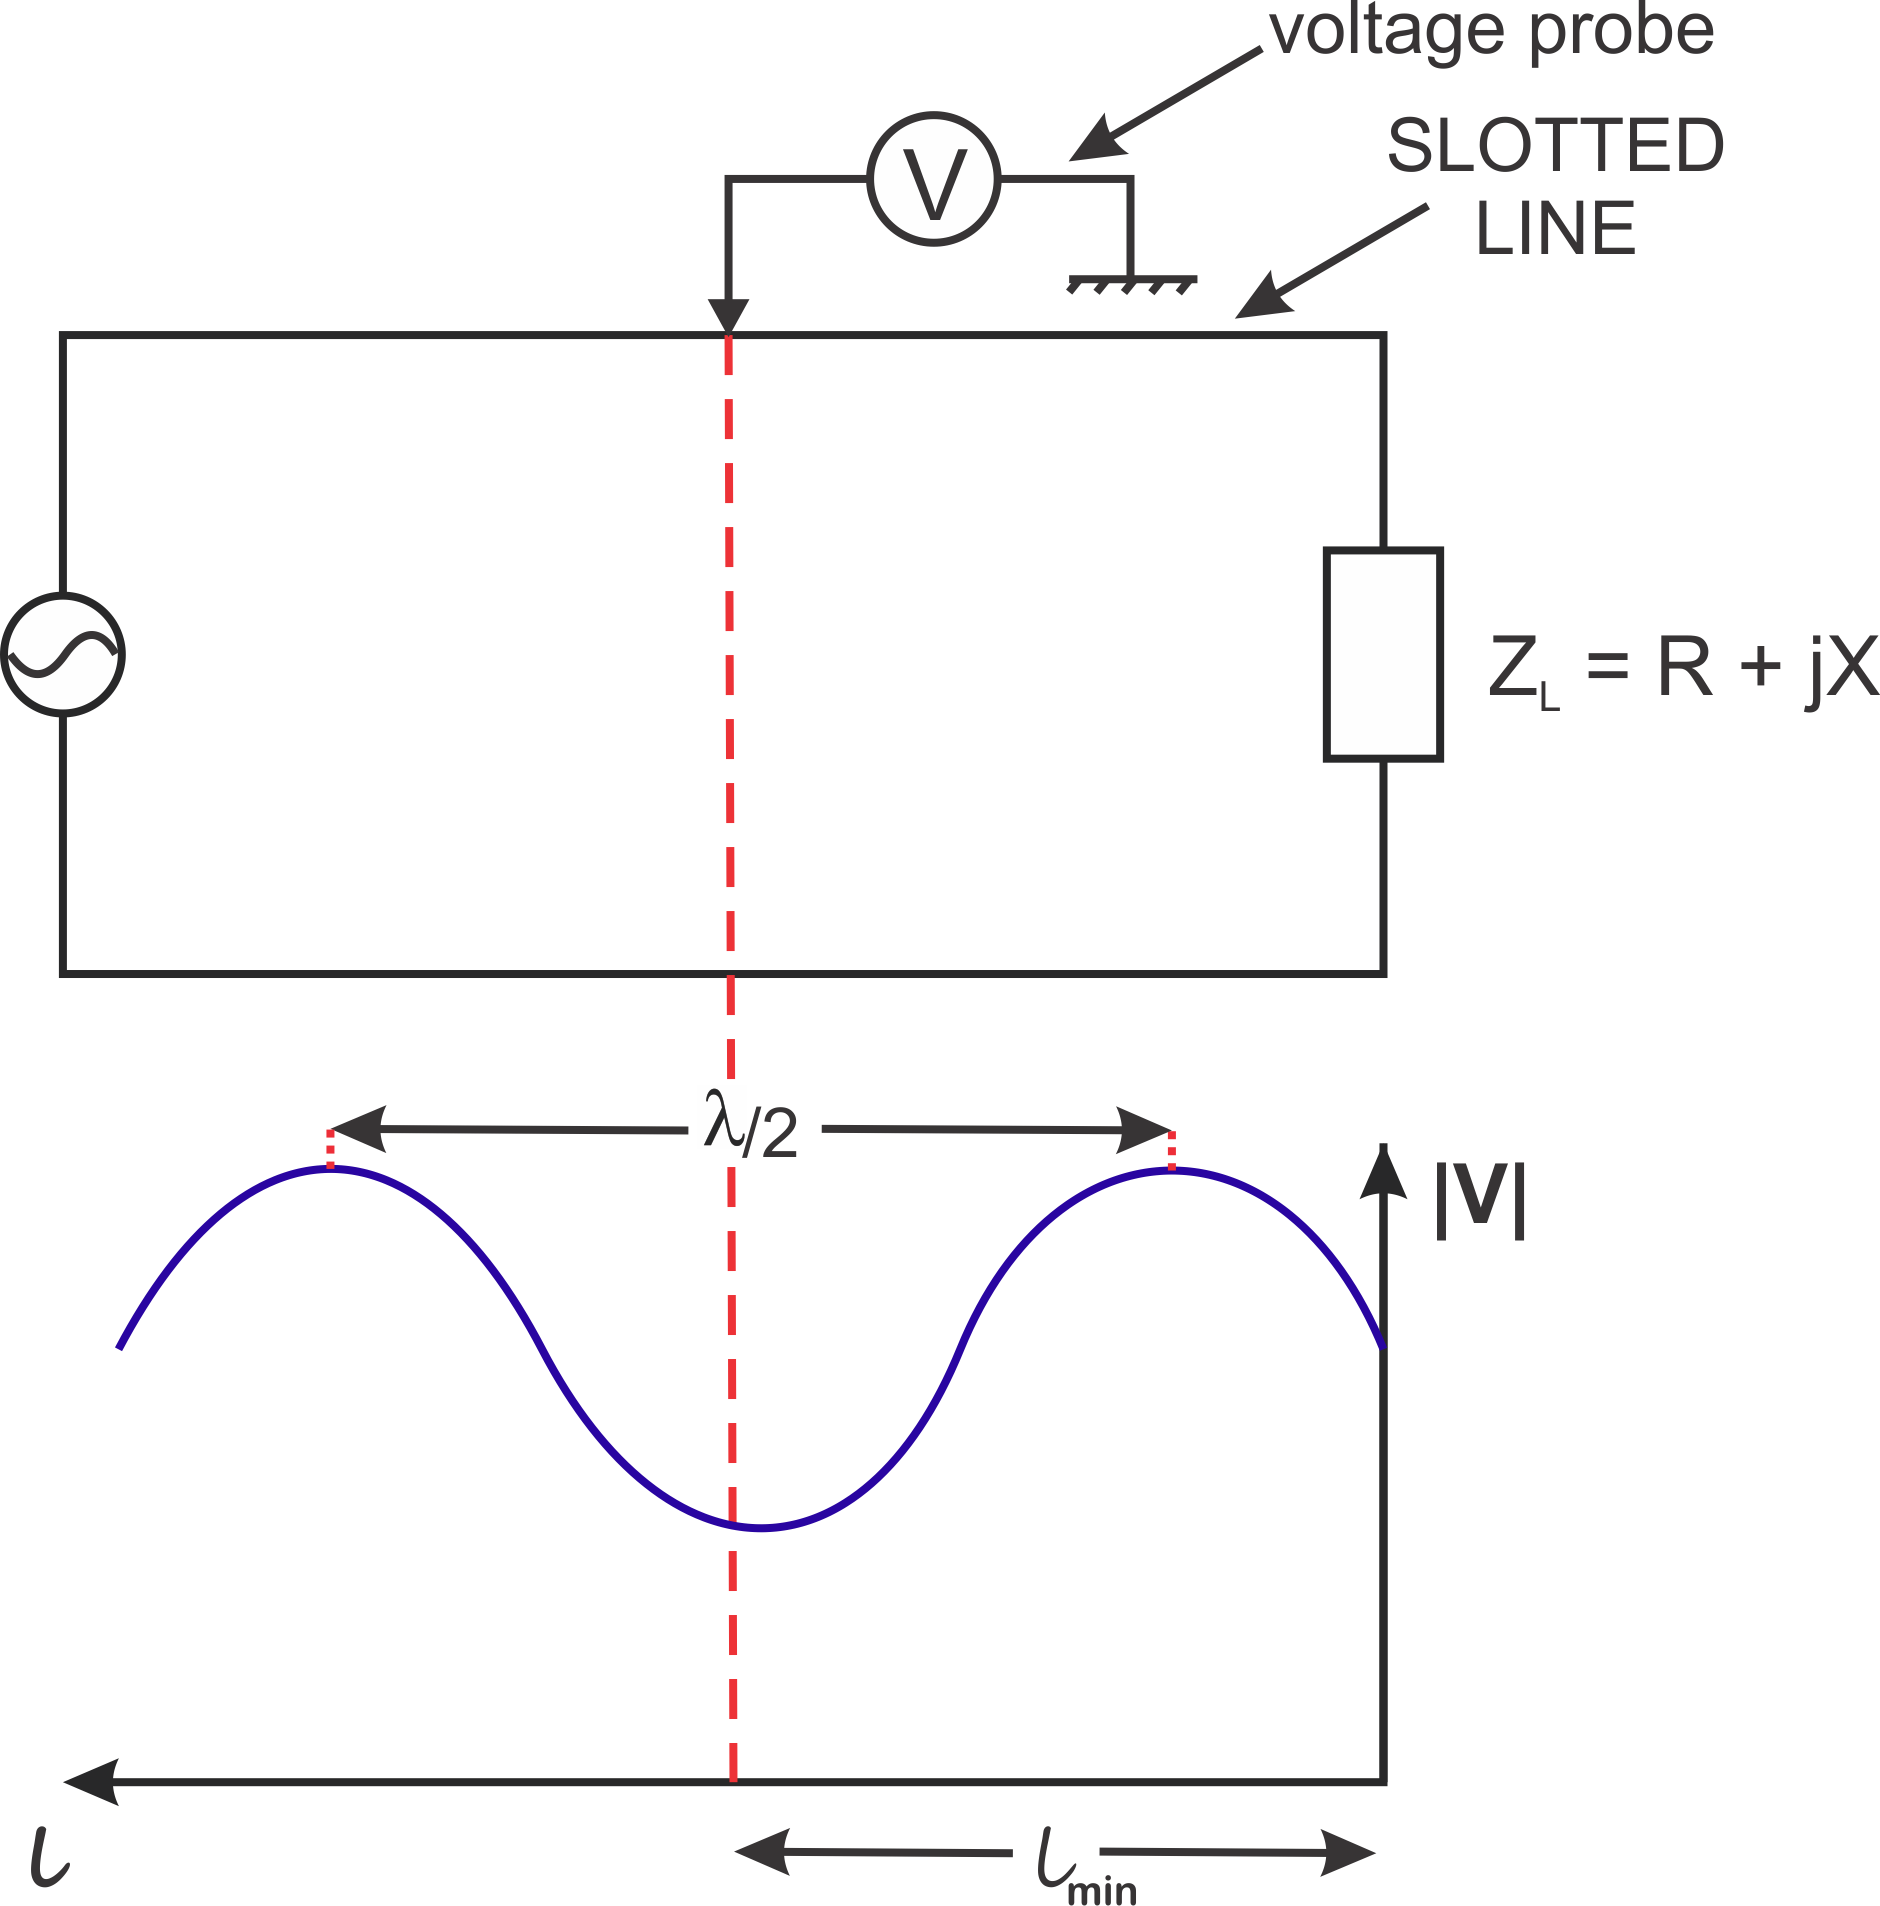
\includegraphics[width=1\linewidth]{./graphics/group10diagram1}
\caption{Measurement using the Slotted Transmission Line}
\end{figure}

The distance between two voltage maxima or minima is $\lambda/2$ and by measuring the separation between two maxima or minima on the transmission line, we can estimate the value of the wavelength. Using the wavelength, we can also find the phase constant $\beta$ since $\beta = 2\pi/\lambda$. The first step in the measurement of unknown impedance is to plot the voltage standing wave pattern, identify the location of two consecutive maxima and minima, measure the distance to estimate $\lambda$, since the distance is $\lambda/2$.

After that, estimate $\beta$ from $\beta$ = $2\pi/\lambda$ . Hence, we measure $l_{min}$, which is the location of the voltage minimum from the the load end of the transmission line. Also we measure $V_{max}$ and $V_{min}$ from the line i.e $|V|_{max}$ and $|V|_{min}$. Since we have measured phase constant $\beta$, $V_{max}$, $V_{min}$, and $l_{min}$. Then we can find out the parameters for impedance calculation. After, we calculate Voltage Standing Wave Ratio (VSWR) for the load.[footnote]
\begin{align}
\rho = \frac{|V|_{max}}{|V|_{min}}
\end{align}

Once we take measurement of $|V|_{max}$ and $|V|_{min}$, then we calculate for $ \rho $. We then find the maximum and minimum impedance which one can see in the Transmission Line. So at $l_{min}$ we have $R_{min}$ at that point and $R_{min}$ = $\frac{Z_o}{\rho}$. Once $R_{min}$ is known at $l_{min}$, the calculation of unknown impedance is simply an impedance transformation problem. We recall that once the impedance at any point on the transmission line is known, the impedance at any other point can be calculated using the impedance transformation relationship.

Since we know $R_{min}$ = $\frac{Z_o}{\rho}$ at $l_{min}$ from the load, we can transform this impedance by a distance $l_{min}$ away from the generator, so that its impedance is equal to terminating impedance $Z_{L}$. So the unknown impedance is nothing but the transformation of $R_{min}$ = $\frac{Z_o}{\rho}$ by $l_{min}$ to the load side of the generator. 
\begin{align}
Z_{L} = Z_o\frac{R_{min}\cos(-\beta l_{min}) + jZ_o\sin(-\beta l_{min})}{Z_o\cos(-\beta l_{min}) + jR_{min}\sin(-\beta l_{min})}
\end{align}
$l_{min}$ is negative since we are moving away from the generator. Finding $Z_{min}$ is a matter of separating the real and imaginary parts, we get the value of resistance and reactance as shown below.\\
\textbf{NOTE:} We are dealing with a lossless transmission line unless otherwise stated.
\begin{dmath}
Z_{L} = Z_o\frac{R_{min}\cos\beta l_{min} - jZ_o\sin\beta l_{min}}{Z_o\cos\beta l_{min} - jR_{min}\sin\beta l_{min}}
\end{dmath}
Rationalize into proper form by multiplying the top and bottom by the conjugate of the denominator.
{\footnotesize 
\begin{dmath}
Z_{L} = Z_o\left(\frac{R_{min}\cos\beta l_{min} - jZ_o\sin\beta l_{min}}{Z_o\cos\beta l_{min} - jR_{min}\sin\beta l_{min}}\right)\times\left(\frac{Z_o\cos\beta l_{min} + jR_{min}\sin\beta l_{min}}{Z_o\cos\beta l_{min} + jR_{min}\sin\beta l_{min}}\right)
\end{dmath}} 
{\footnotesize 
\begin{dmath}
Z_{L} = Z_o
\frac{Z_oR_{min}\cos^{2}\beta l_{min} + Z_oR_{min}\sin^{2}\beta l_{min}}{Z_o^{2}\cos^{2}\beta l_{min} + R_{min}^{2}\sin^{2}\beta l_{min}} +j\frac{(R_{min}^{2}-Z_o^{2})\cos\beta l_{min}\sin\beta l_{min}}{Z_o^{2}\cos^{2}\beta l_{min} + R_{min}^{2}\sin^{2}\beta l_{min}}
\end{dmath}}
Recall $ \cos^{2}(A) + \sin^{2}(A) = 1 $ and $ \frac{\sin(A)}{\cos(A)} = \tan(A) $
\begin{dmath}
Z_{L} = Z_o\frac{Z_oR_{min} + j(R_{min}^{2}-Z_o^{2})\cos\beta l_{min}\sin\beta l_{min})}{(Z_o^{2}\cos^{2}\beta l_{min} + R_{min}^{2}\sin^{2}\beta l_{min})}
\end{dmath}
Divide numerator and denominator by $\cos^{2}\beta l_{min}$:
\begin{align*}
Z_{L} = Z_o\frac{\frac{Z_oR_{min}}{\cos^{2}\beta l_{min}} + \frac{j(R_{min}^{2}-Z_o^{2})\cos\beta l_{min}\sin\beta l_{min})}{\cos^{2}\beta l_{min}}}{\frac{(Z_o^{2}\cos^{2}\beta l_{min} + R_{min}^{2}\sin^{2}\beta l_{min})}{\cos^{2}\beta l_{min}}}
\end{align*}
Recall $ \frac{1}{\cos(A)} = \sec(A) $
\begin{align}
Z_{L} = Z_o\{\frac{Z_oR_{min}\sec^{2}\beta l_{min} + j(R_{min}^{2}-Z_o^{2})\tan\beta l_{min}}{Z_o^{2}+ R_{min}^{2}\tan^{2}\beta l_{min}}\}
\end{align}
$\frac{Z_o}{R_{min}} = \rho$ , Divide numerator and denominator by $R_{min}^{2}$ to have numerator as:
\begin{align*}
Z_{L} = Z_o\{\frac{Z_oR_{min}}{R_{min}^{2}}\sec^{2}\beta l_{min} + \frac{j(R_{min}^{2}-Z_o^{2})}{{R_{min}^{2}}}\tan\beta l_{min}\}
\end{align*}
\begin{align*}
Z_{L} = Z_o [\rho \sec^{2}\beta l_{min} + j(1-\rho^{2})\tan\beta l_{min}] =
\end{align*}
\begin{align*}
Z_{L} = Z_o [ \rho (1 + \tan^{2}\beta l_{min}) + j(1-\rho^{2})\tan\beta l_{min}]
\end{align*}
Denominator changes thus:
\begin{align*}
\frac{1}{R_{min}^{2}}{(Z_o^{2} + R_{min}^{2}\tan^{2}\beta l_{min})} = \rho^{2} + \tan^{2}\beta l_{min}
\end{align*}
We have:
{\footnotesize
\begin{dmath}
Z_{L} = Z_o \left[\frac{\rho (1 + \tan^{2}\beta l_{min}) + j(1-\rho^{2})\tan\beta l_{min}}{\rho^{2} + \tan^{2}\beta l_{min}} \right]
\end{dmath}}
\begin{dmath*}
\overline{Z_{L}} = \frac{Z_{L}}{Z_o} =  \frac{\rho (1 + \tan^{2}\beta l_{min})}{\rho^{2} + \tan^{2}\beta l_{min}} + \frac{j(1-\rho^{2})\tan\beta l_{min}}{\rho^{2} + \tan^{2}\beta l_{min}}
\end{dmath*}

Real Part: $R = Z_o[\frac{\rho (1 + \tan^{2}\beta l_{min})}{\rho^{2} + \tan^{2}\beta l_{min}}]$\\

Imaginary Part: $ X = Z_o[\frac{(1-\rho^{2})\tan\beta l_{min}}{\rho^{2} + \tan^{2}\beta l_{min}}]  $\\

Hence $Z_{L}$ = R +jX can easily be calculated from all parameters that we have measured viz; $|V|_{max}$,$|V|_{min}$, Voltage Standing Wave Ratio $\rho = \frac{|V|_{max}}{|V|_{min}}$, $l_{min}$, $\beta$ from $\beta = 2\pi/\lambda$. Hence, we have transformed $R_{min}$ to $Z_{L}$ without necessarily knowing the value of $R_{min}$, as seen in our expression for X i.e. reactance and R i.e. resistance, where it is not required for the calculation. 
However, in practice, when connecting the unknown impedance to the slotted line section, we use conductors as well as other forms of connectors. This means the location of the impedance is not accurately known, so measurement of $l_{min}$, sometimes become inaccurate. If we know $l_{min}$ precisely, then the solution is straightforward and very accurate in finding out what the unknown impedance is. If $l_{min}$ is not known, there would be error in the unknown impedance.\\

To avoid error, we define the location of the load by replacing it with a short circuit. Carry out the measurement of the transmission line, and find out the location of $l_{min}$ with the line terminated with a short circuit. Then replace the short circuit by a load and find out the new standing wave pattern with the load. So we have two standing wave patterns on our transmission line. 
\begin{enumerate}[(i)]
\item With the line terminated with a short circuit and 
\item with the unknown load terminating the line.
\end{enumerate}
For short circuits, we identify the exact location of minimum voltage by the standing wave, which becomes our origin for the unknown load impedance measurement of $l_{min}$.

Hence the superposition of the load standing wave pattern on the short circuit standing wave is shown above.
\begin{figure}[h]
\centering
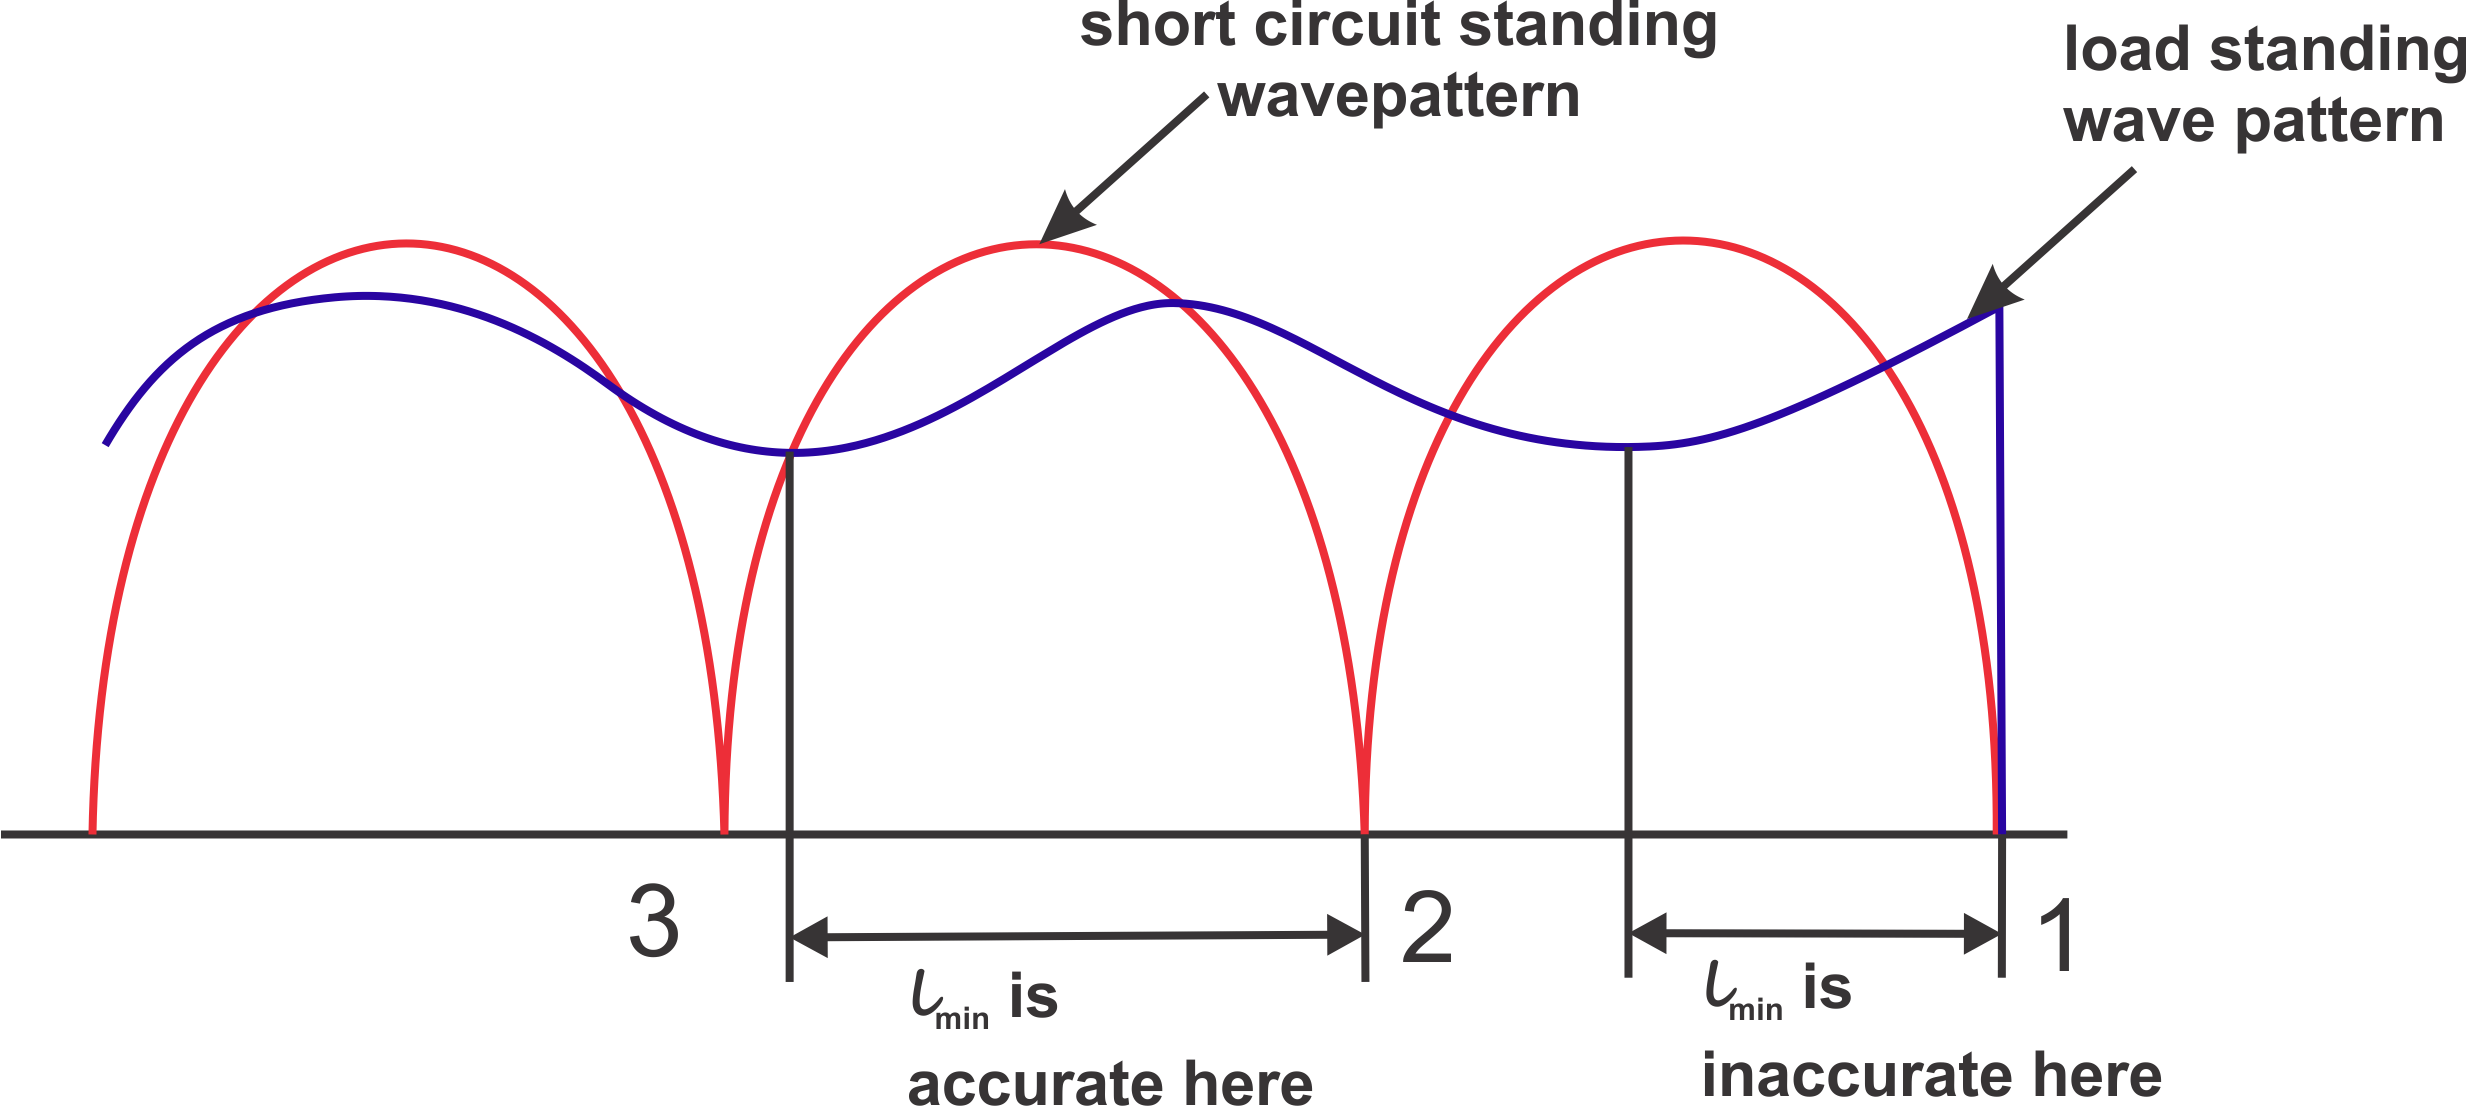
\includegraphics[width=1\linewidth]{./graphics/group10diagram2}
\caption{Superposition of the load standing wave pattern and the short circuit standing wave}
\end{figure}

The minimum voltage for the short circuit standing wave pattern repeats itself at $\lambda/2$, so we can start our measurement at position 1, 2, or 3 and measure the corresponding load $l_{min}$ from either of these points towards the left. So instead of starting measurement at position 1 which was not accurate because of conductors used in the connection or the presence of connectors, we can start from 2 or 3 as origin and  then measure $l_{min}$ of the load that occur after the first point.\\
In practice, to find $l_{min}$, we take the measurement for both short circuit and the unknown load standing
wave patterns, to remove the inaccuracies introduced by the connecting conductors or connectors.\newline

This technique of impedance measurement is very useful. In fact at high frequencies (e.g. microwave frequencies) without measurement like this on a slotted line, one will not be able to measure the unknown impedance. So at high frequency, the Transmission line is suitable for the measurement of unknown impedance.
The second application for Transmission line is as a \textbf{circuit element}.

\section{ Transmission Line as circuit element}
Assuming we wound the inductor as shown below at high frequency which have inductance L. At high frequency, there is a capacitance between the turns of the inductor that almost short out current as $X_{C} = \frac{1}{2\pi fc}$. This was not case at low frequency when the turns appeared separated from one another. Hence, at high frequency we then have distributed capacitors between the turns of inductor.
\begin{figure}[h]
\centering
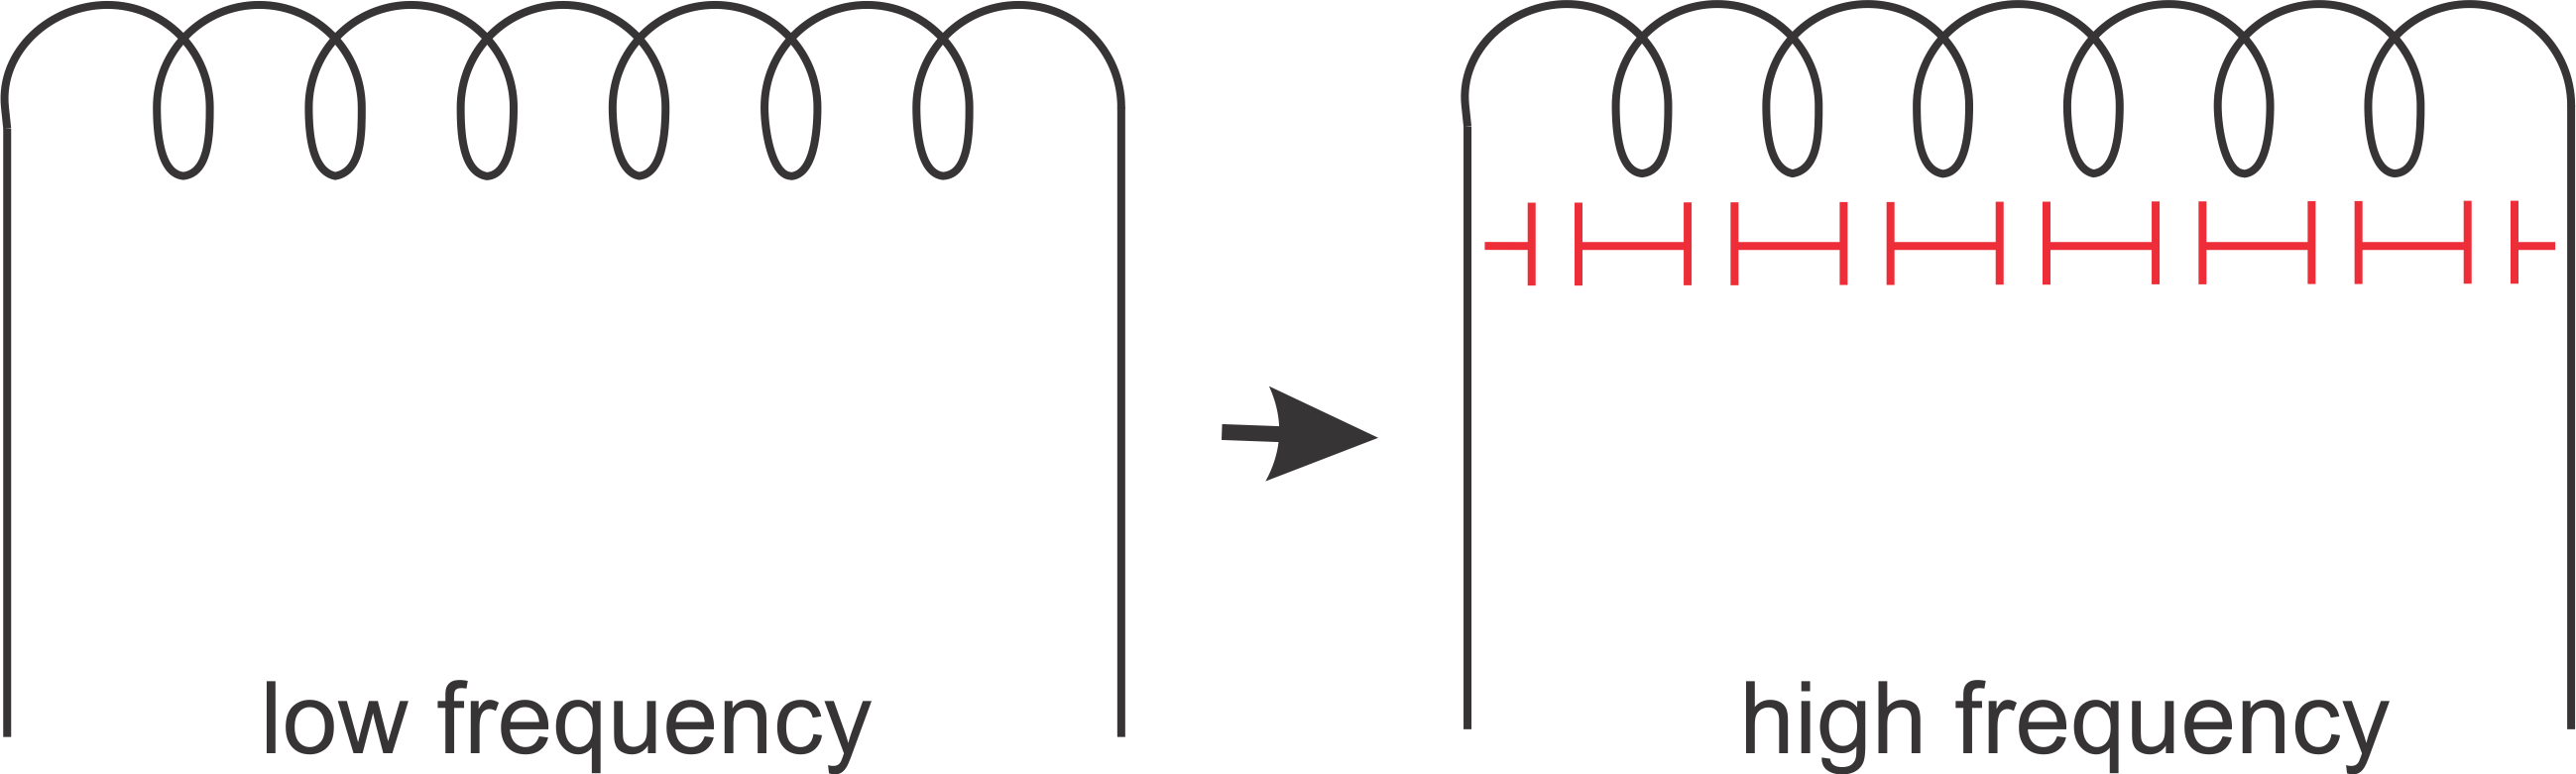
\includegraphics[width=1\linewidth]{./graphics/group10diagram3}
\caption{An inductor at Low frequency and then at High frequency}
\end{figure}

As the frequency increases, the inductor starts having capacitive reactance. It shows for typical wire wound inductor, the resonance frequency lies for distributed capacitances and inductances in the range of 100 - 200MHz.
It means if we wound an inductor, beyond about few 100MHz, the inductor will not exhibit its ideal characteristics, rather like that of a capacitor because we have already crossed the resonance frequency. So the effect of capacitance is more dominant compared to the inductance.

Similarly, suppose we take a capacitor at low frequency, it will exhibit its ideal characteristics. As the frequency increases, the connecting leads or wires which have inductance starts to predominate beyond certain frequencies, the capacitor no longer exhibit its ideal characteristics.
\begin{figure}[h]
\centering
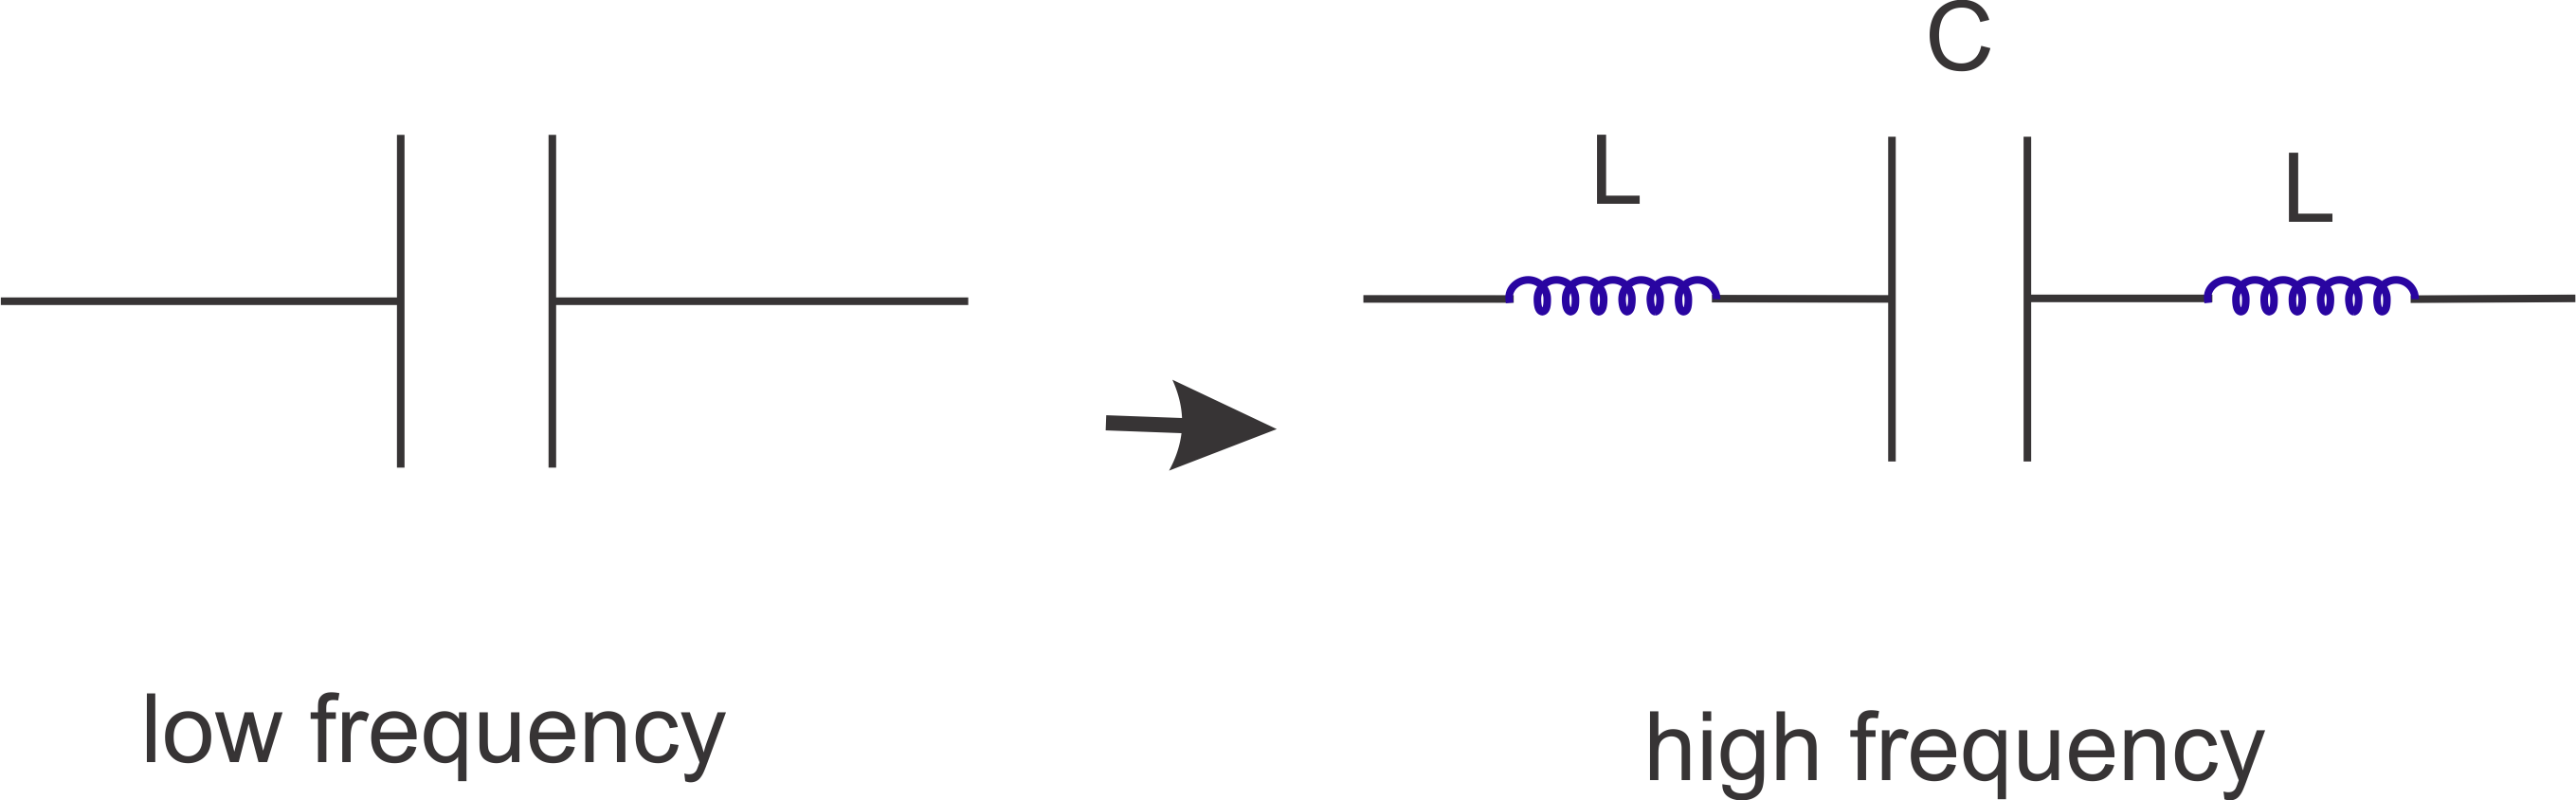
\includegraphics[width=1\linewidth]{./graphics/group10diagram4}
\caption{An capacitor at Low frequency and then at High frequency}
\end{figure}

Hence we can reliably design an inductor at low frequencies. But at high frequencies, its reliability is very poor because the inductor is no longer ideal. Similarly for a capacitor at high frequencies, the lead inductance starts to predominate and the capacitor no longer exhibit its ideal characteristics. So at high frequency, realizing a reactive element is not that easy because, we do not have a reliable circuit element which will guarantee its use as a capacitor or inductor. When the frequency is increasing, the wavelength is becoming smaller as we have seen earlier. 
If you consider a short or open circuit line, the input impedance of these lines would behave like a reactance.

So as the frequency increases and the wavelength getting smaller, the size of a transection (a small lineal element) of a transmission line which can give you impedance which is reactive, becomes more physically realizable.
Two things have become clear when working with transmission
Lines;
\begin{enumerate}[(i)]
\item The lumped circuit are becoming more difficult to realize at high frequency.
\item Realization of reactance by using transmission lines section is becoming easier, because the wavelength is becoming smaller and sections of the transmission line are becoming more feasible.
\end{enumerate}
At high frequency, most reactive sections are replaced by transmission line.
\begin{figure}[h]
\centering
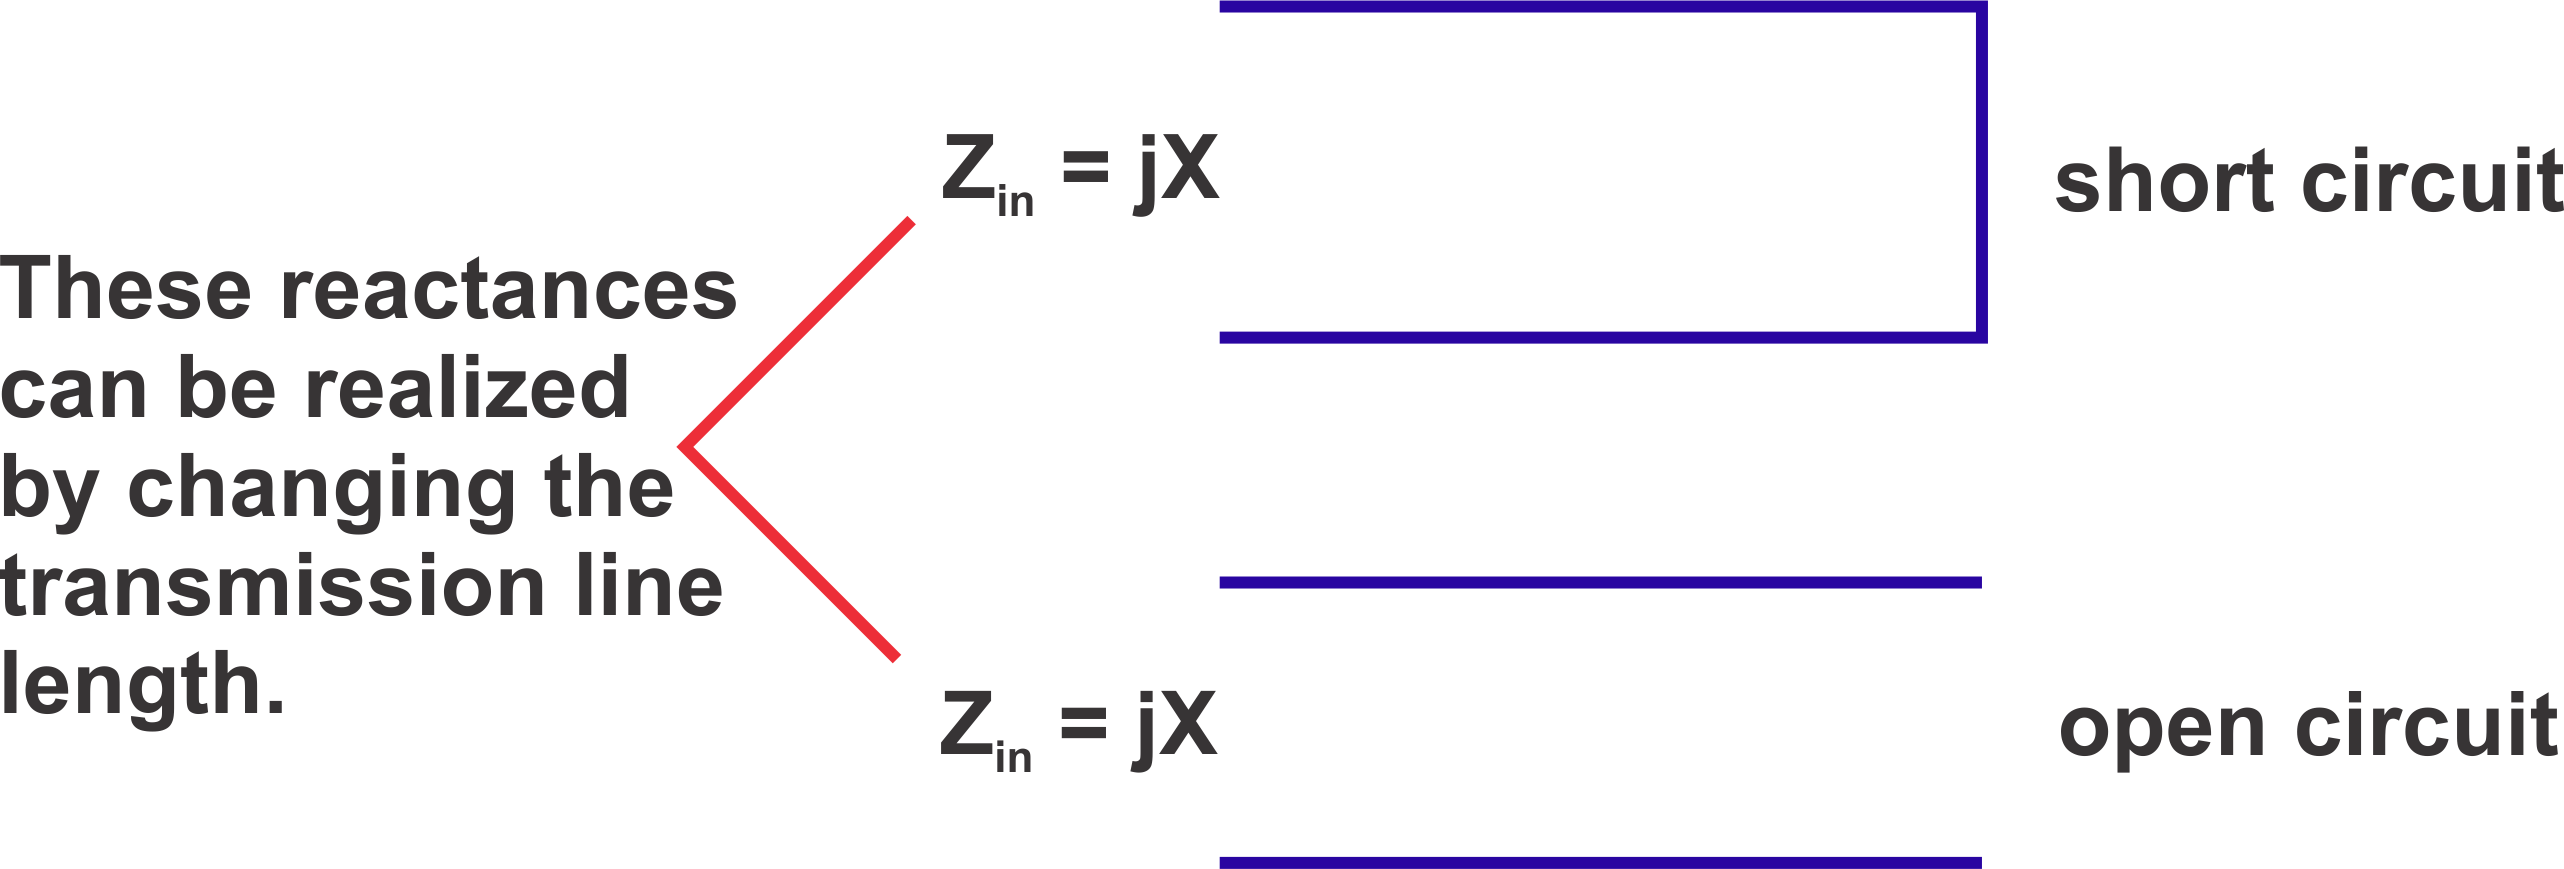
\includegraphics[width=1\linewidth]{./graphics/group10diagram5}
\caption{Transmission Line as a Circuit element}
\end{figure}

In the impedance Smith chart, open circuit is to the right and
short circuit is to the left on the outermost circle. Moving along
the outermost circle which has r = 0 implies we are tracing
out pure reactance. Moving clockwise in this outermost circle,
shows how much length (in terms of wavelength) you move from
the load towards the generator, so that at any point on this outer
circle, we get a pure reactance. We can assume the presence of
that reactance at that point, from the open or short circuit end
towards the signal source or generator.
Hence for a load of open or short circuit, by using different length of transmission line, we can get different reactance at the input. So the question is what should be the length of the transmission line, so that one gets a particular value of reactance at the input?\\
Analytically,
$ l $ is the distance towards the generator.\\ Recall for a LOSSLESS Transmission Line which we assume unless stated otherwise.
\begin{align*}
Z_{L} = Z_o \{ \frac{Z_{L}\cos\beta l + jZ_o\sin\beta l}{Z_o\cos\beta l + jZ_{L}\sin\beta l}\}  
\end{align*}
\begin{center}
$Z_{L} = 0$ for short circuit 
\end{center}
\begin{align}
Z_{L} = Z_o \{ \frac{0 + jZ_o\sin\beta l}{Z_o\cos\beta l + 0}\}  = jZ_o\tan\beta l
\end{align}
\begin{align*}
Z_{L} = Z_o \{ \frac{Z_{L}\cos\beta l + jZ_o\sin\beta l}{Z_o\cos\beta l + jZ_{L}\sin\beta l}\}  
\end{align*}
\begin{center}
$Z_{L} = \infty$ for open circuit. Limit equation, since it tends to infinity. 
\end{center}
\begin{align*}
Z_{L} = Z_o \{ \frac{\cos\beta l + j\frac{Z_o}{Z_{L}}\sin\beta l}{\frac{Z_o}{Z_{L}}\cos\beta l + j\sin\beta l}\}  
\end{align*}
\begin{align}
Z_{L} = Z_o \{ \frac{\cos\beta l + j \times 0}{0 + j\sin\beta l}\} = -jZ_o\cot\beta l  
\end{align}
\begin{center}
$ Z_{(L)} = jZ_o\tan\beta l \Rightarrow $ short circuit\\ 
\end{center}

\begin{center}
$ Z_{(L)} = -jZ_o\cot\beta l \Rightarrow $ open circuit
\end{center}
Hence the problem of realizing a given reactance from open or short circuit load is to just find $ l $ to get the appropriate $Z_{(L)}$. 
Let $l_{SC}$ and $l_{OC}$ represent short circuit and open circuit length respectively, then we have $ X = jZ_o\tan\beta l_{sc} $ and $ X = -jZ_o\cot\beta l_{oc} $ for short circuit and open circuit respectively. Since the phase constant $ \beta $ is known for the transmission line, we make $ l_{SC} $ and $ l_{OC} $ the subject of the formula, we already know the reactance (X) we require, so that 
\begin{align}
l_{SC} = \frac{1}{\beta}\tan^{-1}\frac{X}{Z_o}, l_{OC} = \frac{1}{\beta}\cot^{-1}\frac{-X}{Z_o}
\end{align}

If the frequency of operation as well as velocity of the wave propagation is known, then we can find $\lambda$ and use $ \beta = \frac{2\pi}{\lambda} $. So we can realize the unknown reactance from using sections of the transmission line. For this calculation, the use of Smith Chart comes in handy. The top half of the impedance Smith Chart at the 
outermost circle is pure inductance, and the bottom half is for capacitance.
However, before we get into details of Smith chart usage, we have to be sure that $ X = Z_o\tan\beta l_{SC} $ and $ X = -Z_o\cot\beta l_{OC} $ for all variation of $ \beta l_{SC} $  from 0 to $ 2\pi $, either $ \tan\beta l_{SC} $ or $ \cot\beta l_{OC} $ varies from $ -\infty$ to +$\infty $.\\

It means if we change the values of $ l_{SC} $ or $ l_{OC} $ in the Transmission line, then we can realize any arbitrary value of the reactance. There is no limit to this. So any value of reactance between $ -\infty$ to $+\infty $ can be realized either by short circuited line or open circuited line. The choice of which one to be used whether short circuit or open circuit line, will depend upon the system you want to employ the circuit element.
For example supposing we have a parallel wire transmission line, then connecting the two ends of the transmission line is rather easy, as we can short the end of the transmission line.\\

However, a transmission line like a Printed Circuit Board (PCB), with ground plane on one side and the line on top separated by a dielectric. To short circuit the line, we will have to drill holes into the Printed Circuit Board using a via, so realizing a short circuit line on that configuration is rather difficult. An open circuit line is preferred. There may be situations where the short circuit line will be preferred over the open circuit line and vice versa. Irrespective of the one used, we will be able to realize all the reactances from  $ -\infty$ to $+\infty $, i.e we can realize any capacitive or inductive reactance by using an open circuited or short circuit section of a transmission line.\\

To find the length, the problem is the opposite of impedance calculation.  Since we know the input impedance $ Z_{in} $ at generator end  and we know terminating impedance ($ Z_{L} $) at the end of the transmission line to be 0 or $ \infty $ whether it is short circuit or open circuit point. We want to find $ l_{SC} $ or $ l_{OC} $, the impedances are known and we want to find the length.
On the Smith chart, mark normalized impedance ($ \overline{Z_{in}} $) position, and note how much should be moved away from short circuit point $ l_{SC} $ or open circuit point $ l_{oc} $, to get to the short circuit point or open circuit point in counter clockwise direction (since we are moving away from the generator).
\begin{figure}[h]
\centering
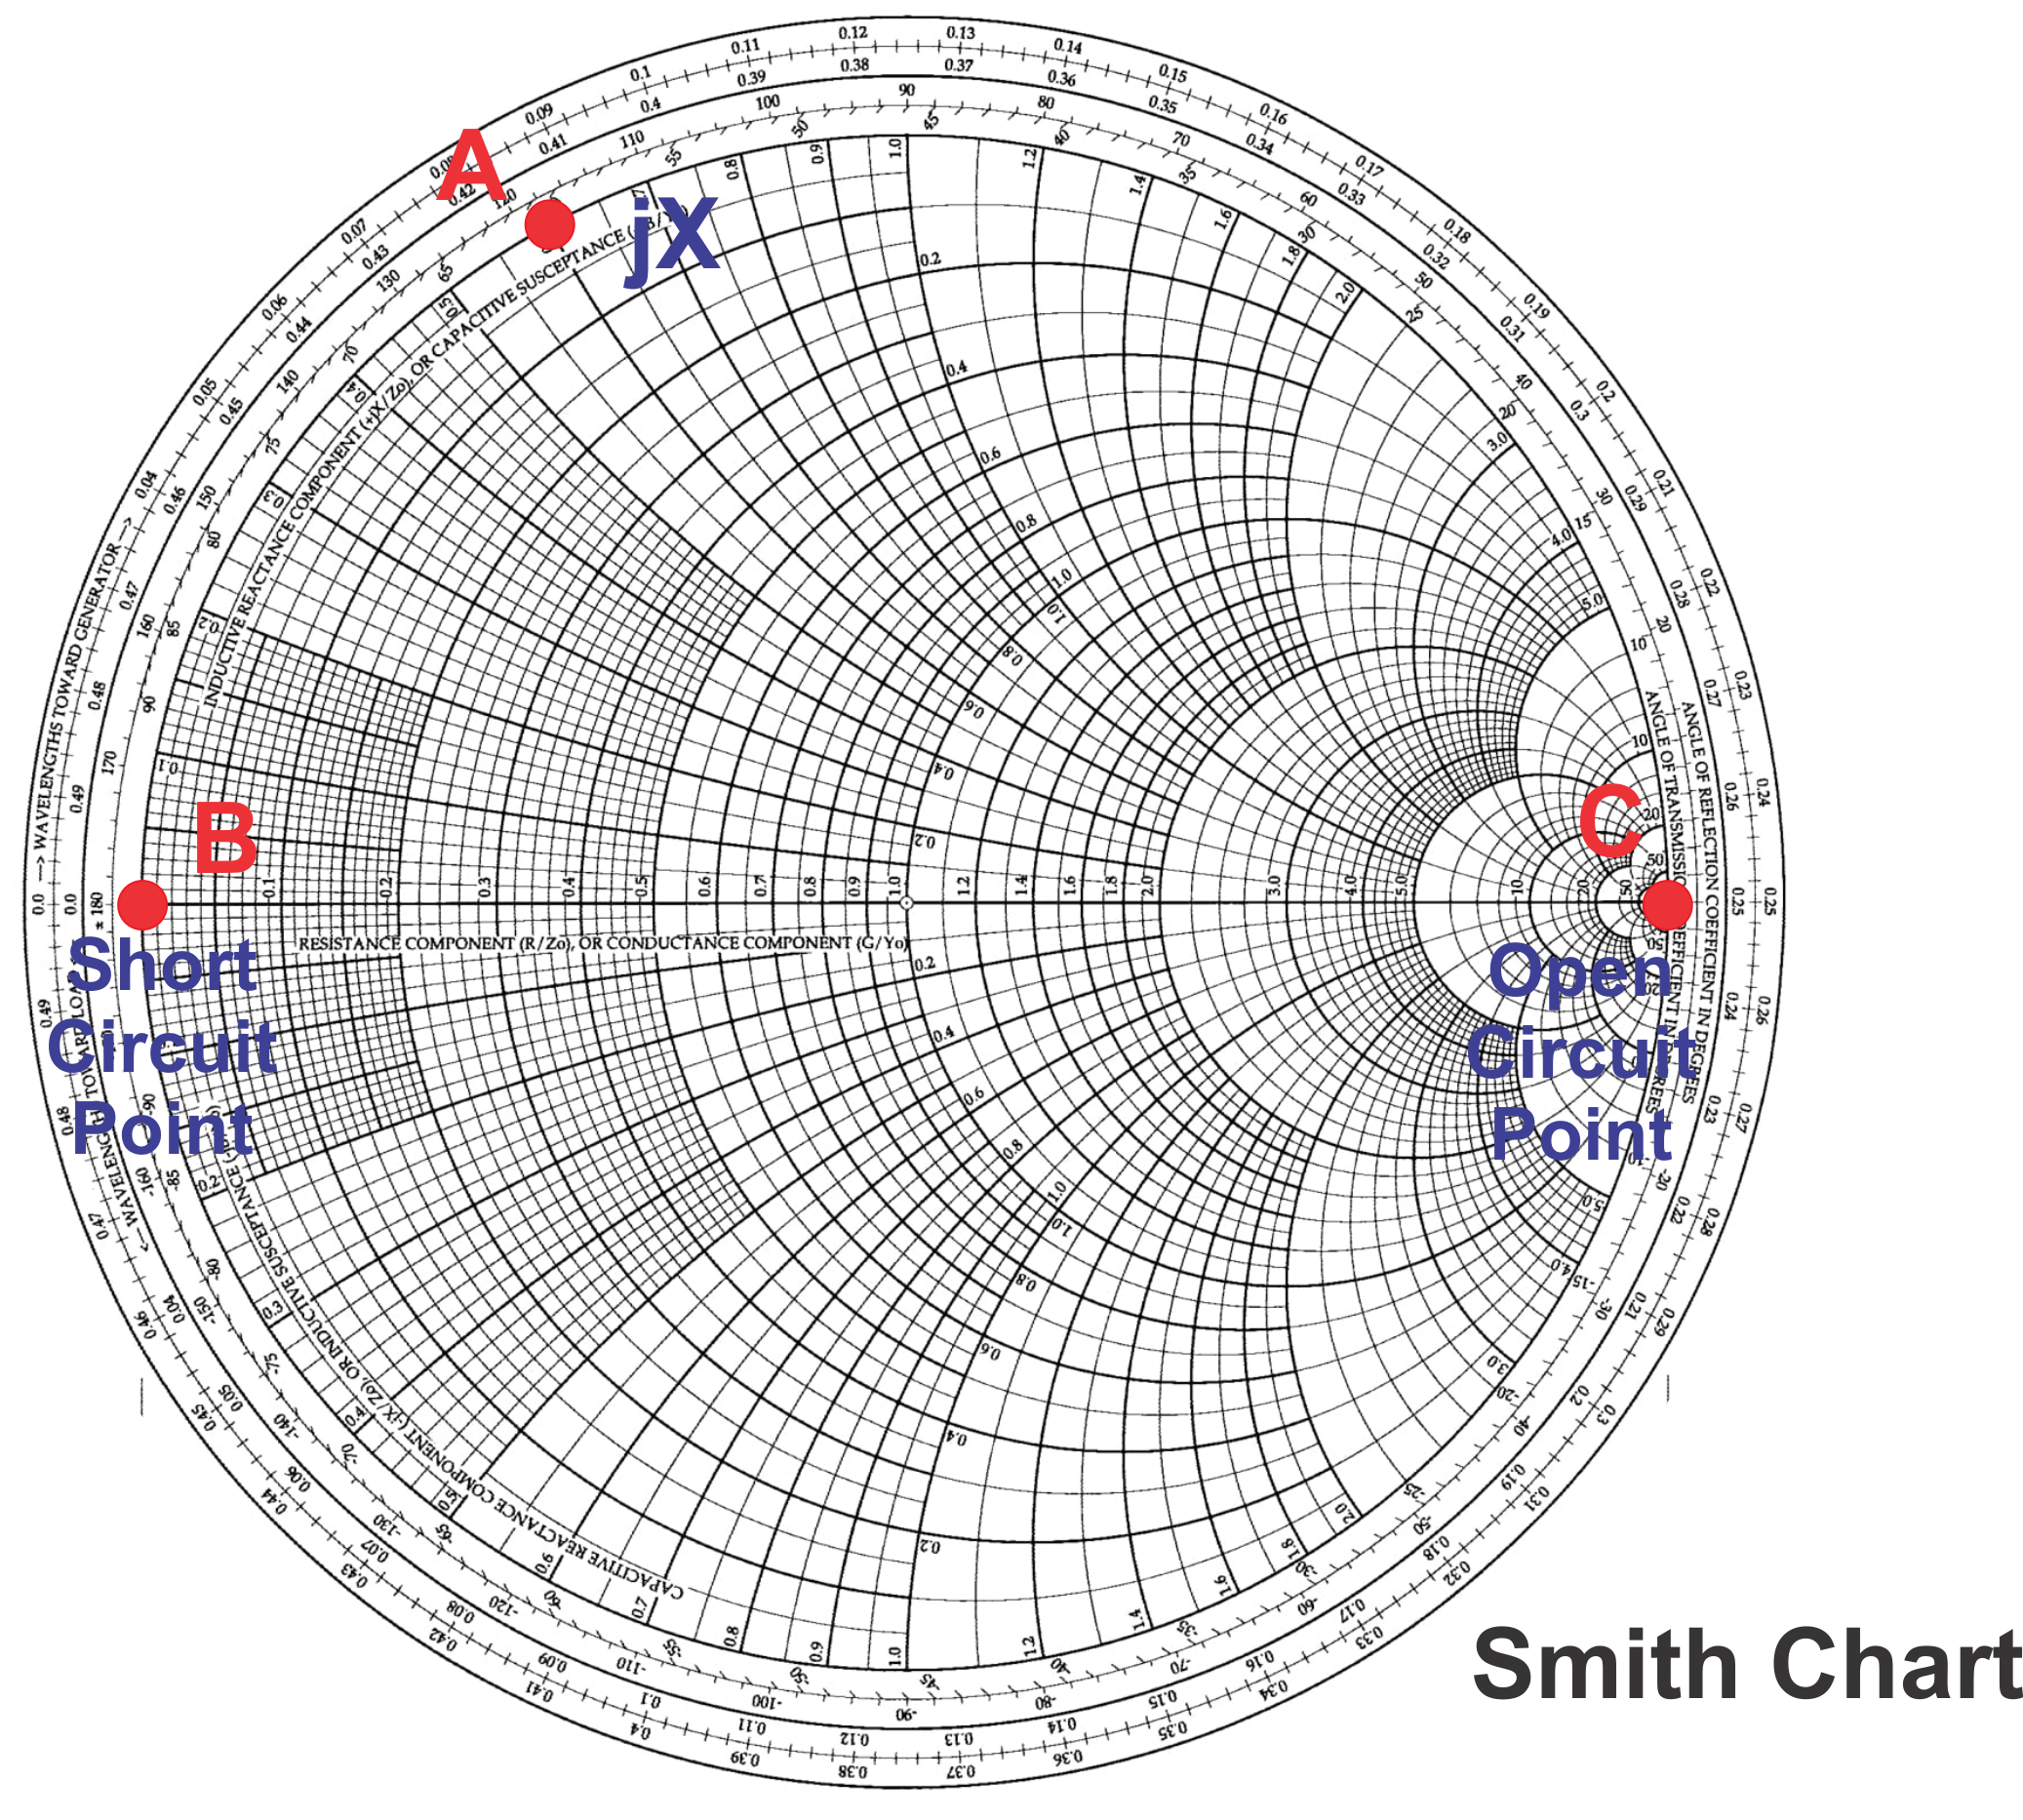
\includegraphics[width=1\linewidth]{./graphics/group10diagram6}
\caption{Open and Short Circuit points on the SMith Chart}
\end{figure} 

Moving away from the generator to reach the short circuit point, means moving counter clockwise from A till we reach B which is the short circuit point. On the Smith chart, clockwise movement is towards the generator and anticlockwise movement is away from the generator.\\Remember on the Smith chart we always use NORMALIZED values. Hence $ \overline{X} $ not X. To realize a capacitive reactance which will be located at the bottom half of the Smith chart for a start.
So that we have,
\begin{figure}[h]
\centering
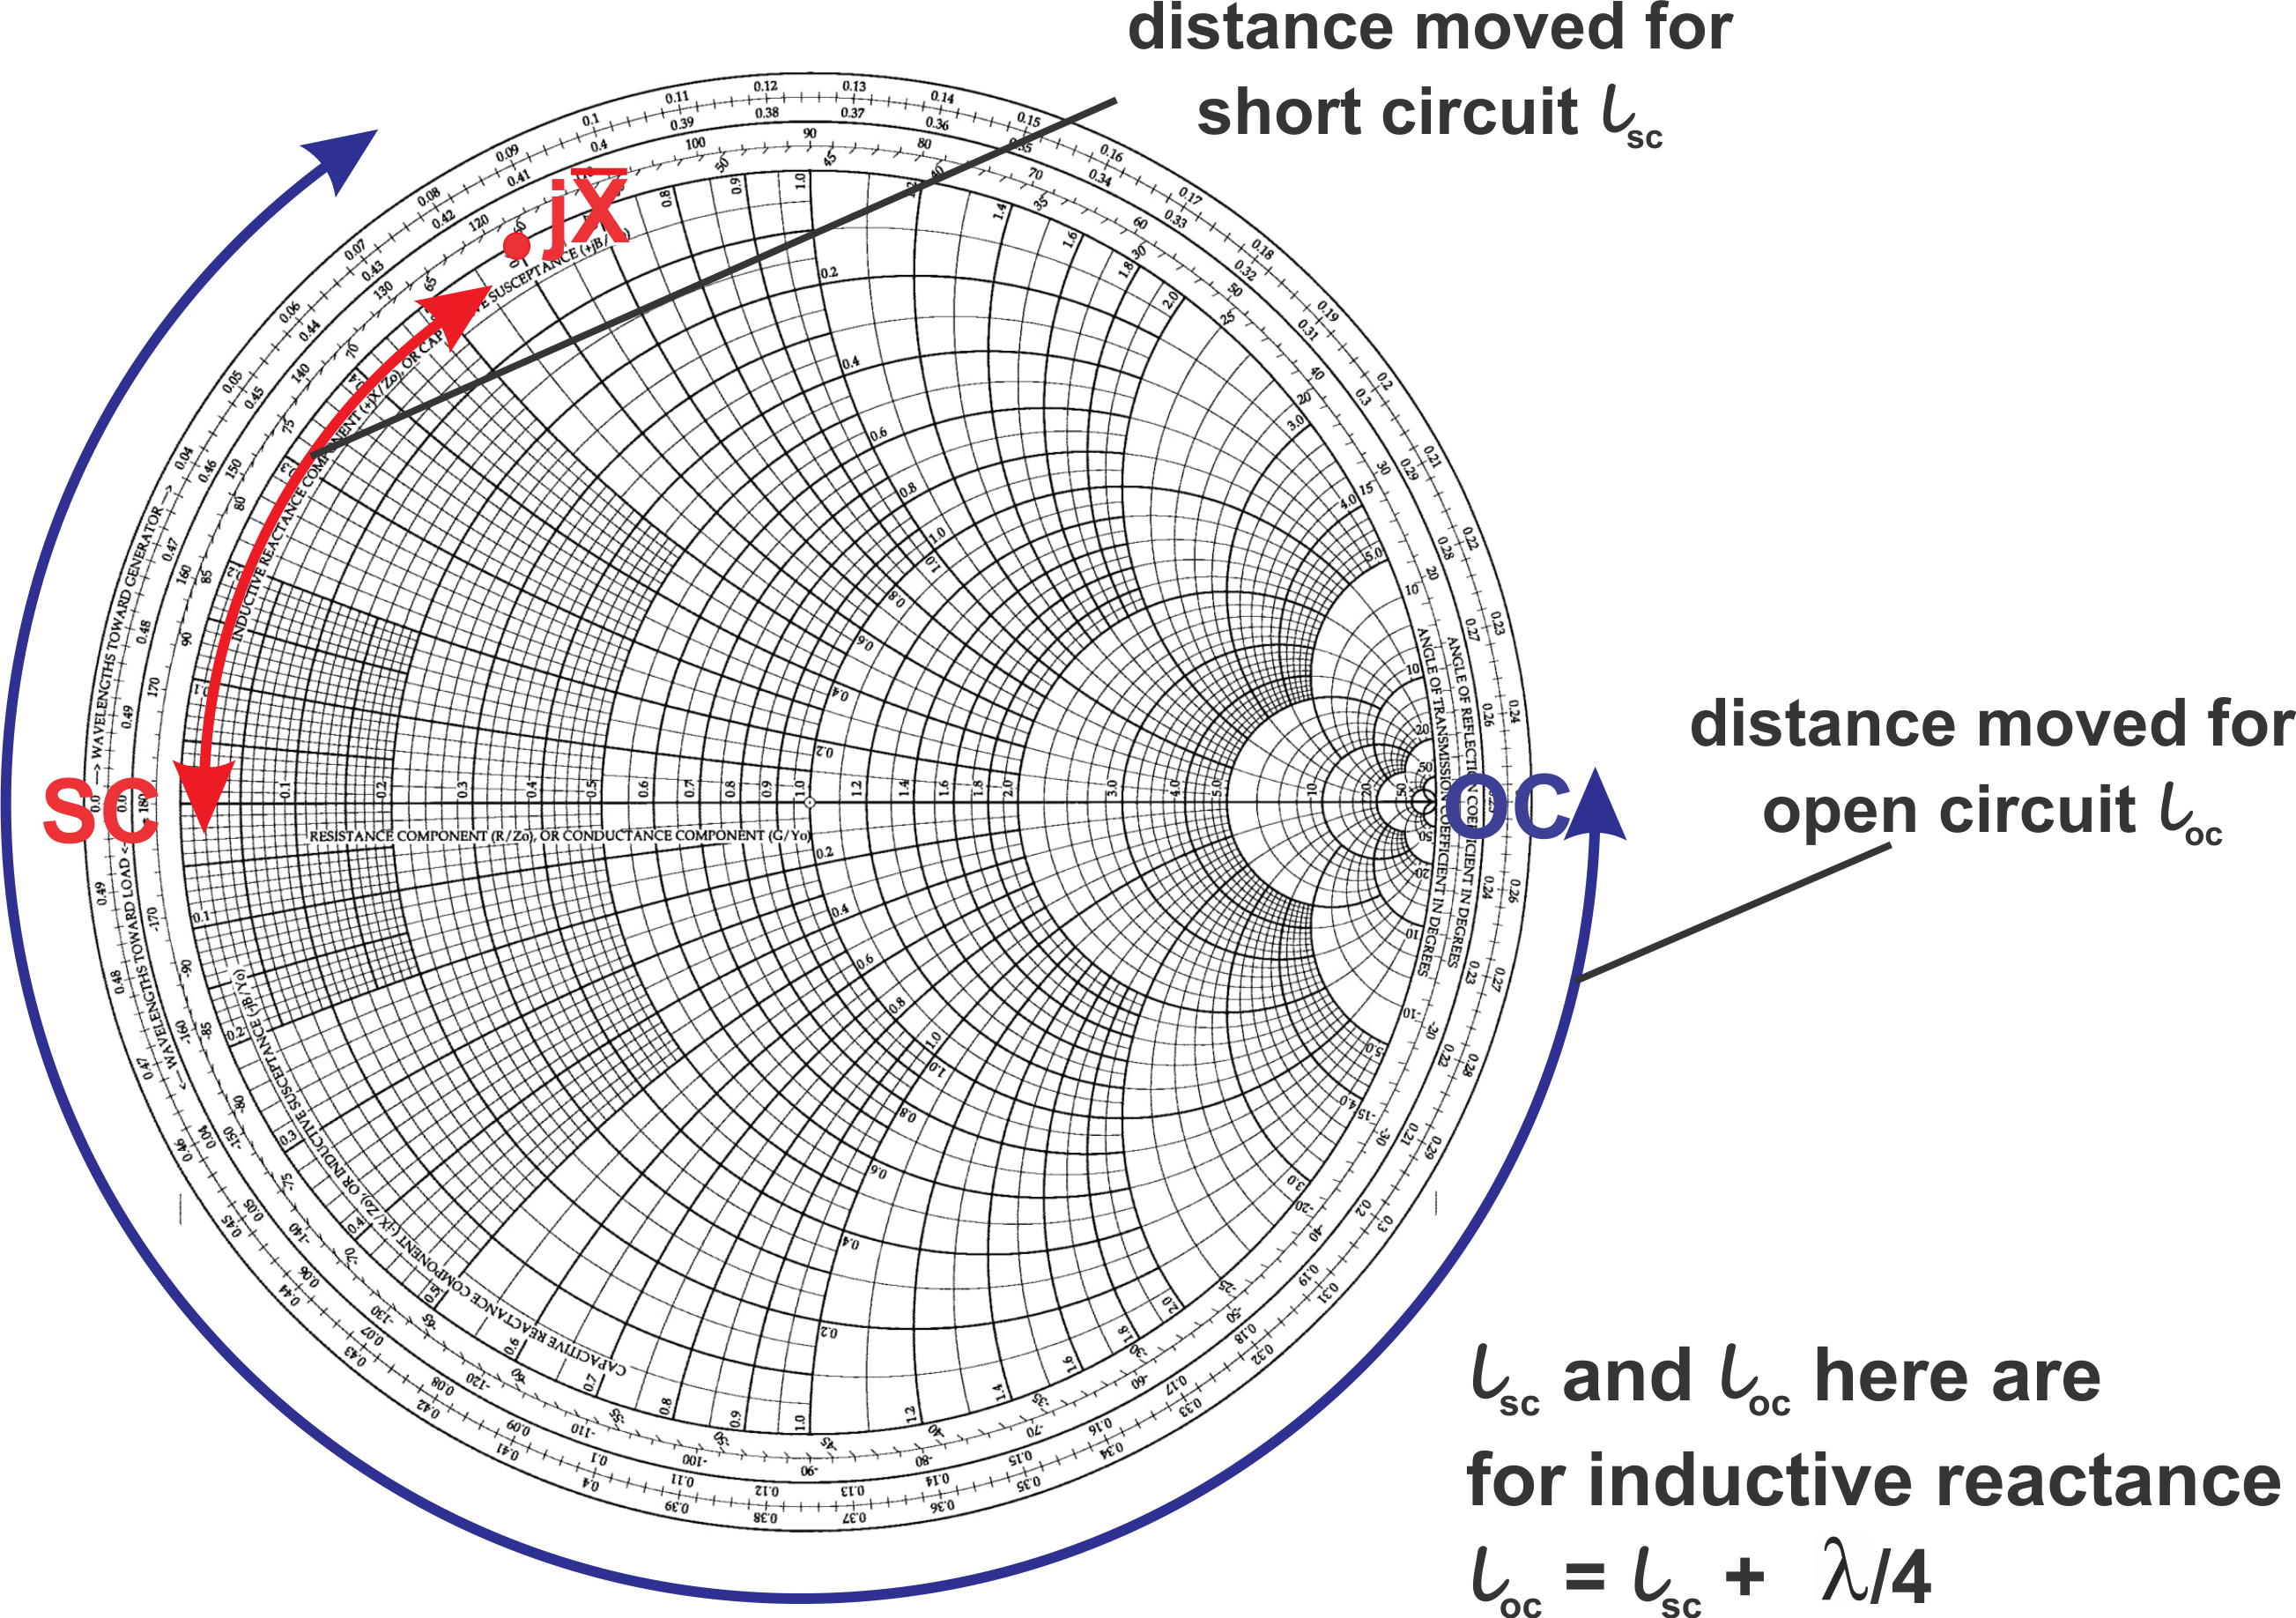
\includegraphics[scale=0.4]{./graphics/group10diagram7}
\caption{$ l_{sc} $ and $ l_{oc} $ for inductive reactance on the smith chart.}
\end{figure}

\begin{figure}[h]
\centering
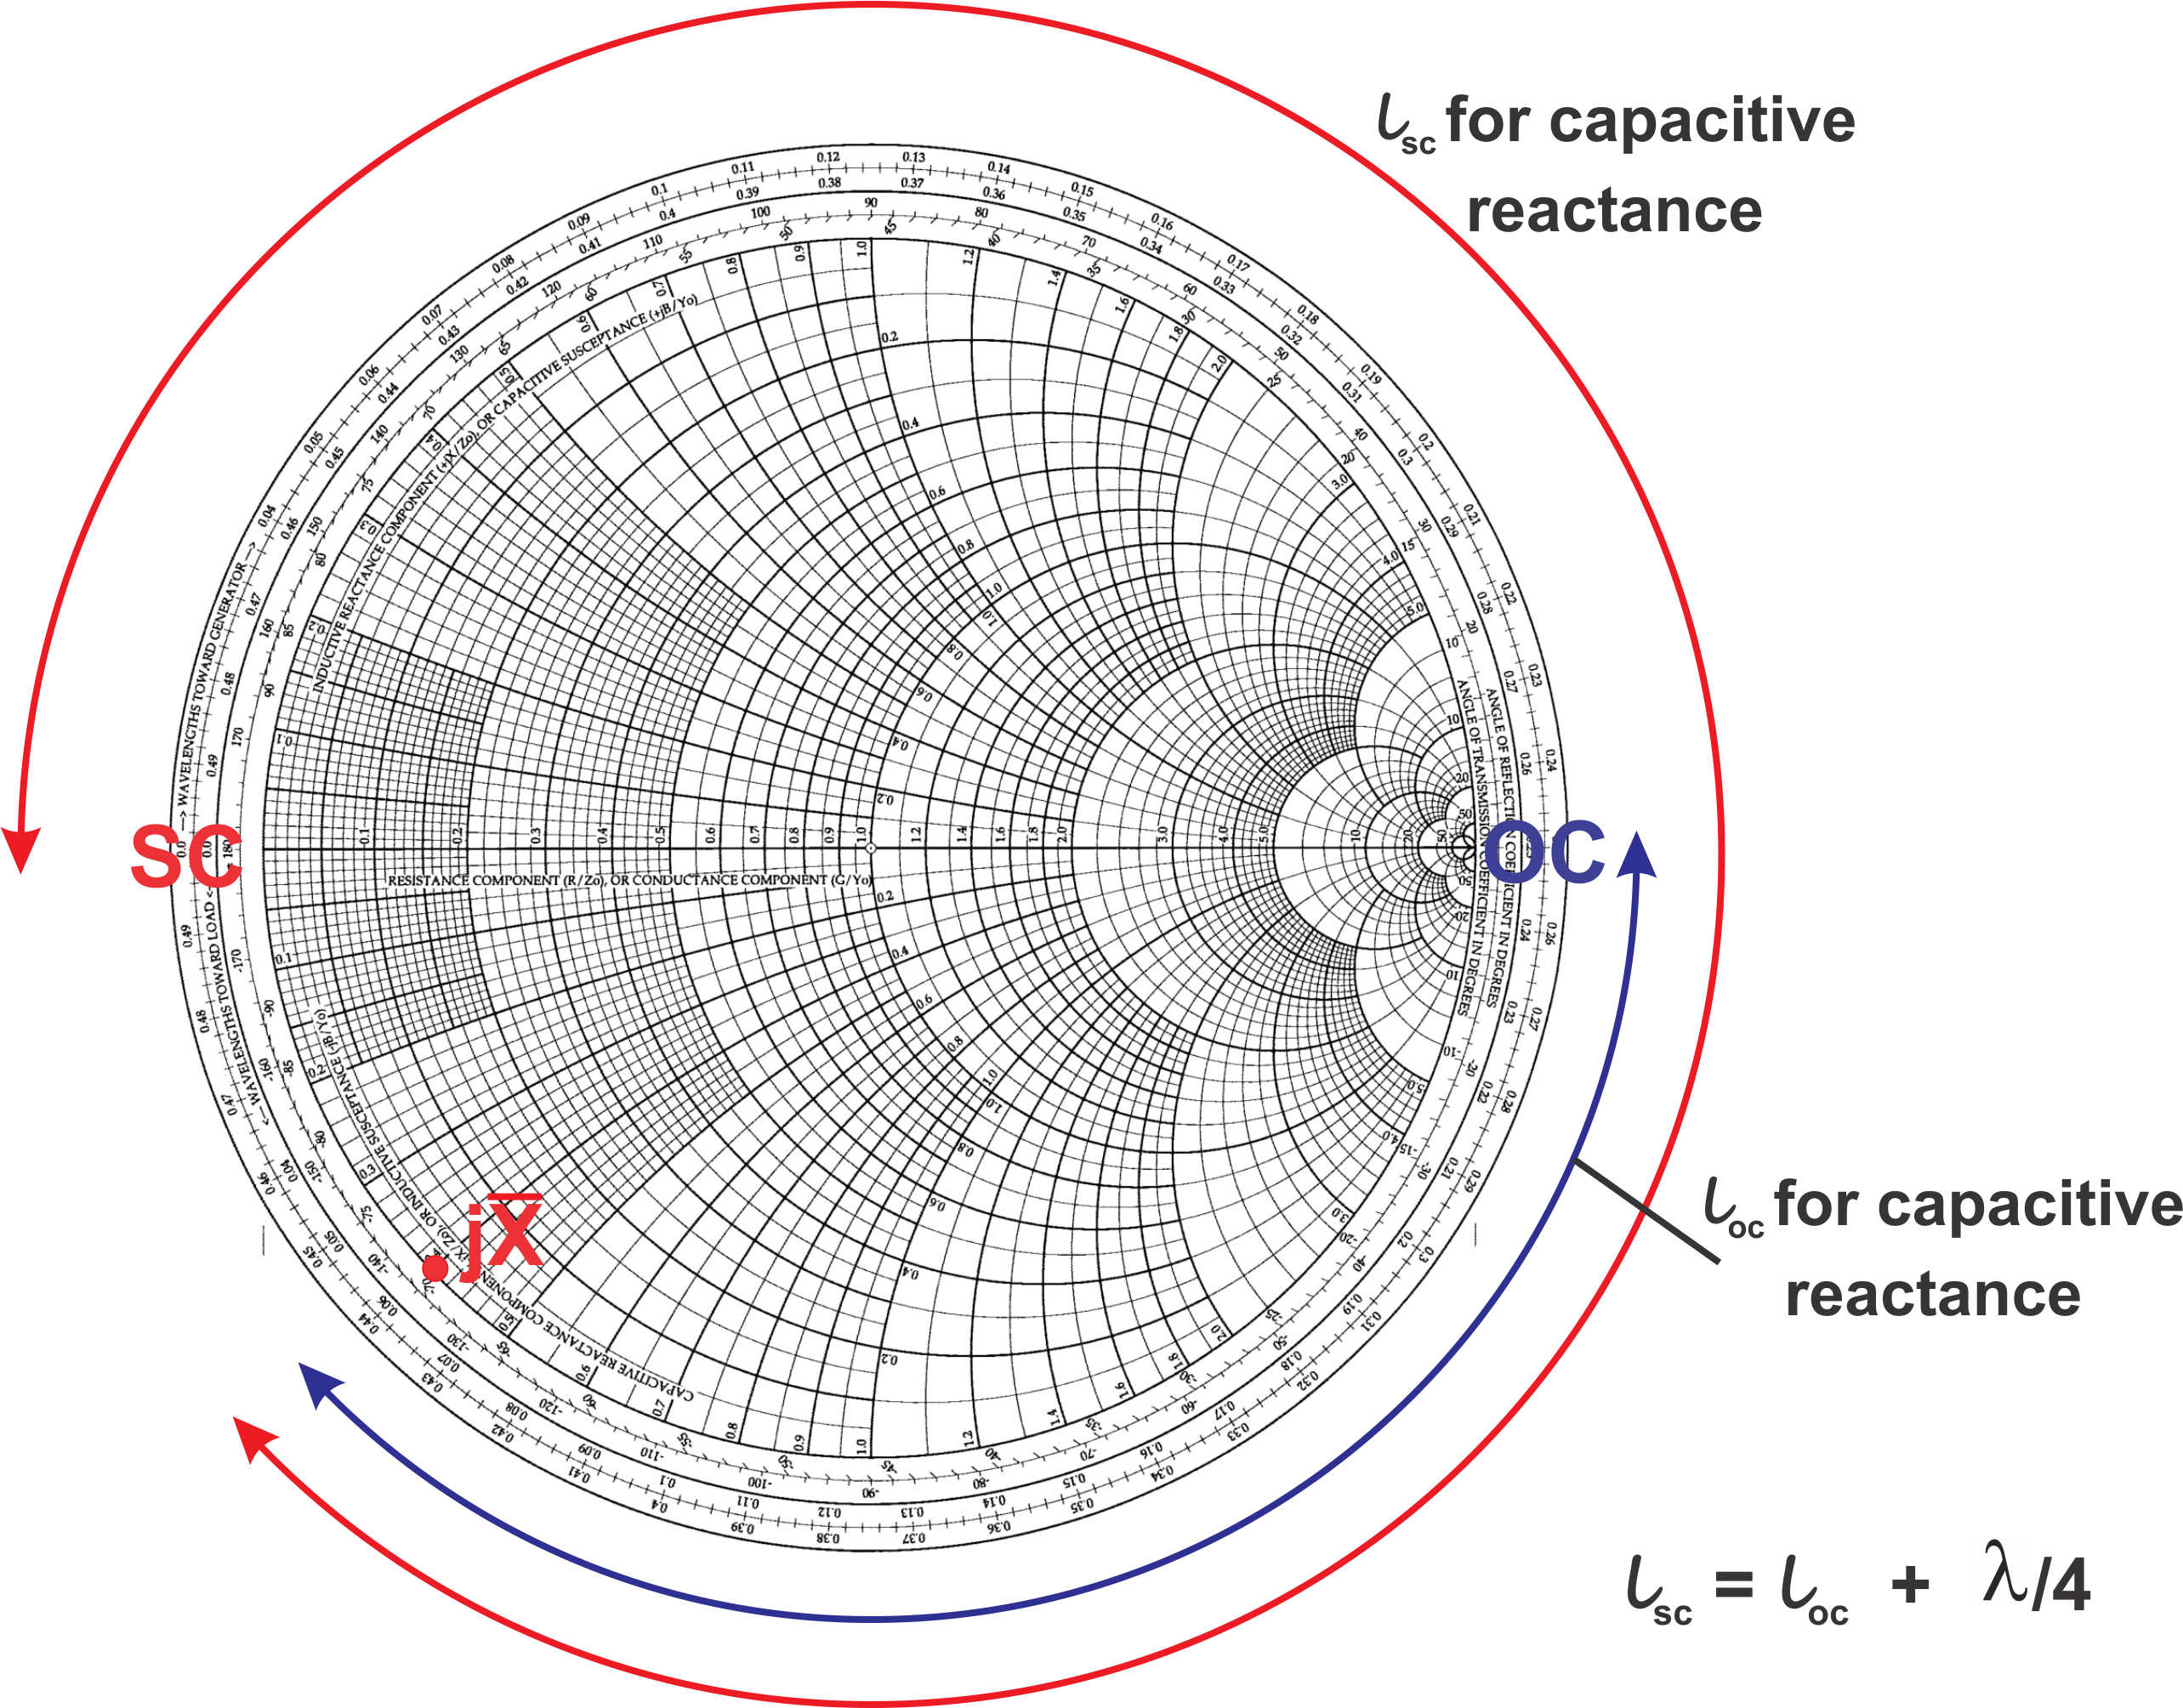
\includegraphics[scale=0.4]{./graphics/group10diagram8}
\caption{$ l_{sc} $ and $ l_{oc} $ for capacitive reactance on the smith chart}
\end{figure}

Moving clockwise from Short circuit \textbf{SC} point by $ \frac{\lambda}{4} $ we have inductive reactance, but beyond that point from $ \frac{\lambda}{4} $ to $ \frac{\lambda}{2} $ we have capacitive reactance. Hence if the length lies within 0 and $ \frac{\lambda}{4} $ for a short circuited line, we have inductive reactance while if the length lies from $ \frac{\lambda}{4} $ to $ \frac{\lambda}{2} $ we have capacitive reactance.
Similarly for an open circuit line moving towards the generator, if  the length lies within 0 to $ \frac{\lambda}{4} $, gives us capacitive reactance and if it lies within $ \frac{\lambda}{4} $ to $ \frac{\lambda}{2} $ we have inductive reactance. It can be written explicitly in the form of diagram below:
\begin{figure}[h]
\centering
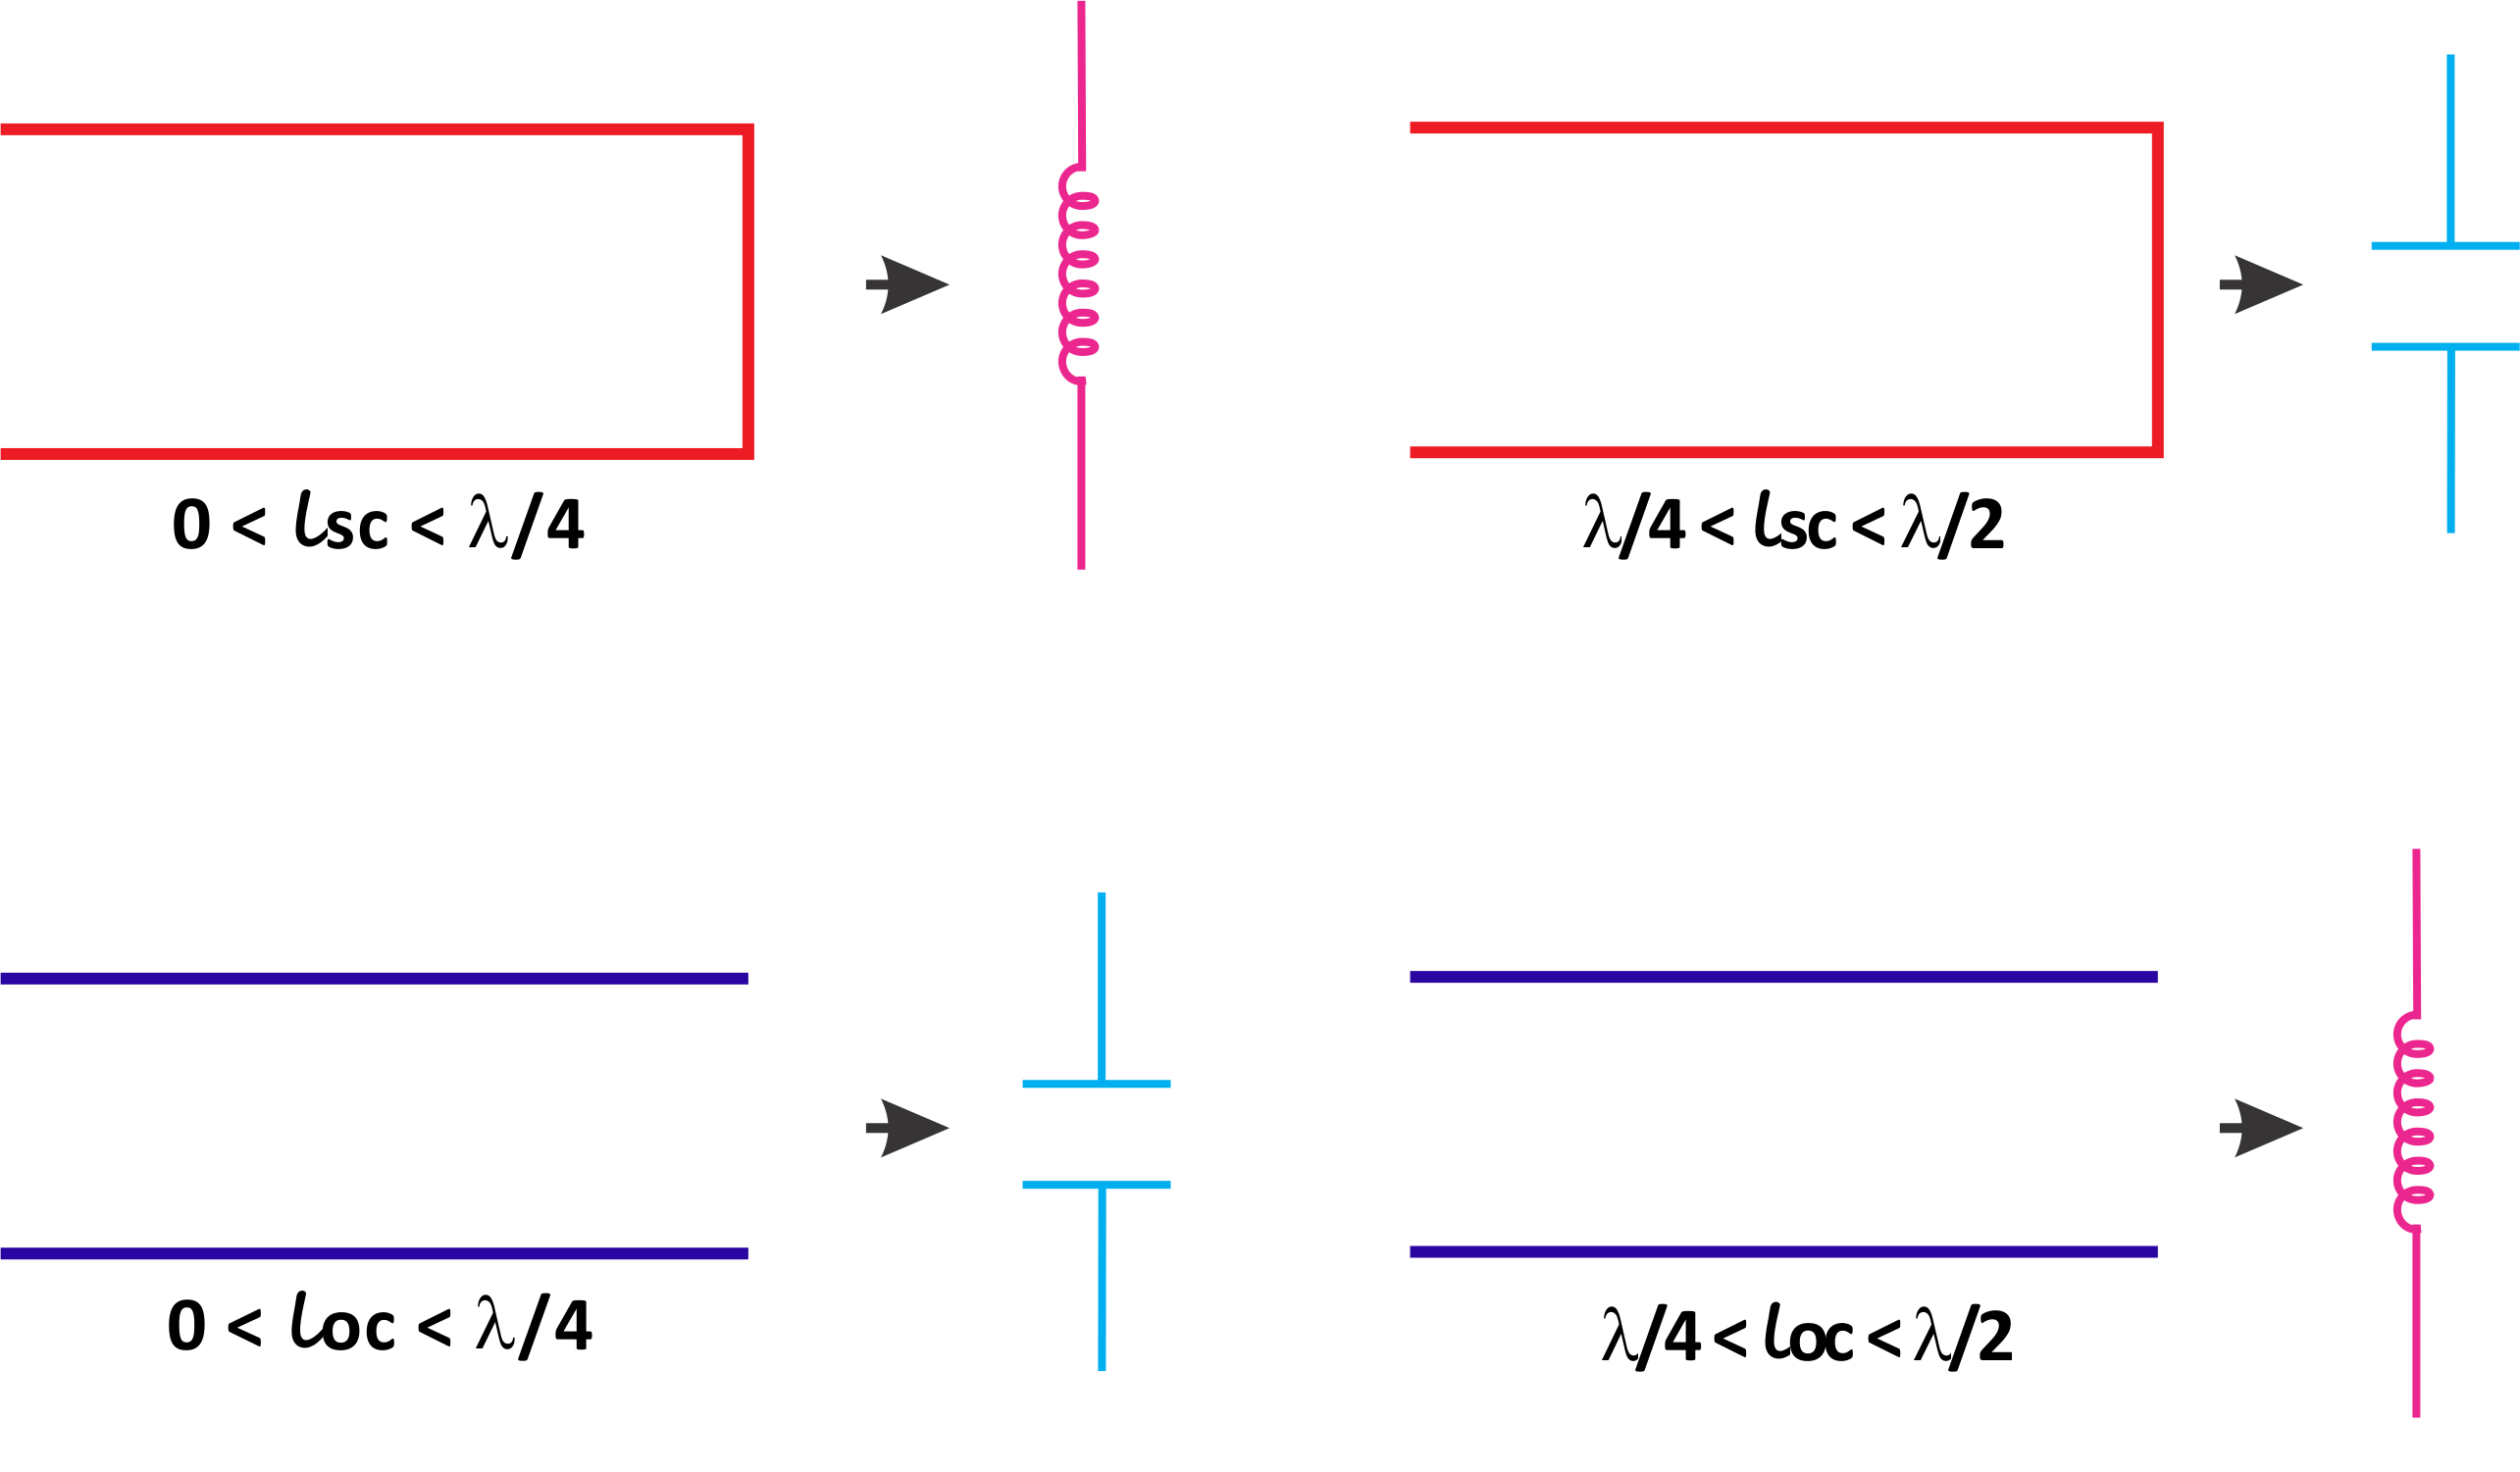
\includegraphics[width=1\linewidth]{./graphics/group10diagram9}
\caption{Nature of impedance for $ l_{sc} $ and $ l_{oc} $ after moving the different lengths}
\end{figure}

So any section of a transmission line of size 0 to $ \frac{\lambda}{2} $ can realize any arbitrary value of capacitance and inductance at a particular frequency. We are not realizing a capacitor or inductor in actual sense, but we are realizing capacitive and inductive reactance. So at $ \frac{\lambda}{4} $ the behavior of the line changes from $ X_{L} $ to $ X_{C} $ or $ X_{C} $ to $ X_{L} $. At $\frac{\lambda}{4}$  location, we have a characteristics that is more like resonance characteristics. Taking a circuit for instance, at resonant frequency \footnote{Resonance frequency is a frequency point where the inductive reactance of the inductor becomes equal in value to the capacitive reactance of the capacitor \textbf{$ X_{L} = X_{C} $}}, on one side you have inductive behavior while on the other side you have capacitive behavior. 

So a section of a transmission line may not only be used as a reactive element, it can also be used as a resonant LC circuit\footnote{It consist of an inductor and capacitor connected together. It is used for generating signals at a particular frequency or picking out a signal at a particular frequency from a more complex signal}. Now we see that suppose you take a line at $ \frac{\lambda}{4} $ to $ \frac{\lambda}{2} $, they will have behavior similar to the LC resonant circuit.\newline
It means that if we change the frequency for a given length of a transmission line, the impedance seen between the terminals of the line is going to change.
\begin{figure}[h]
\centering
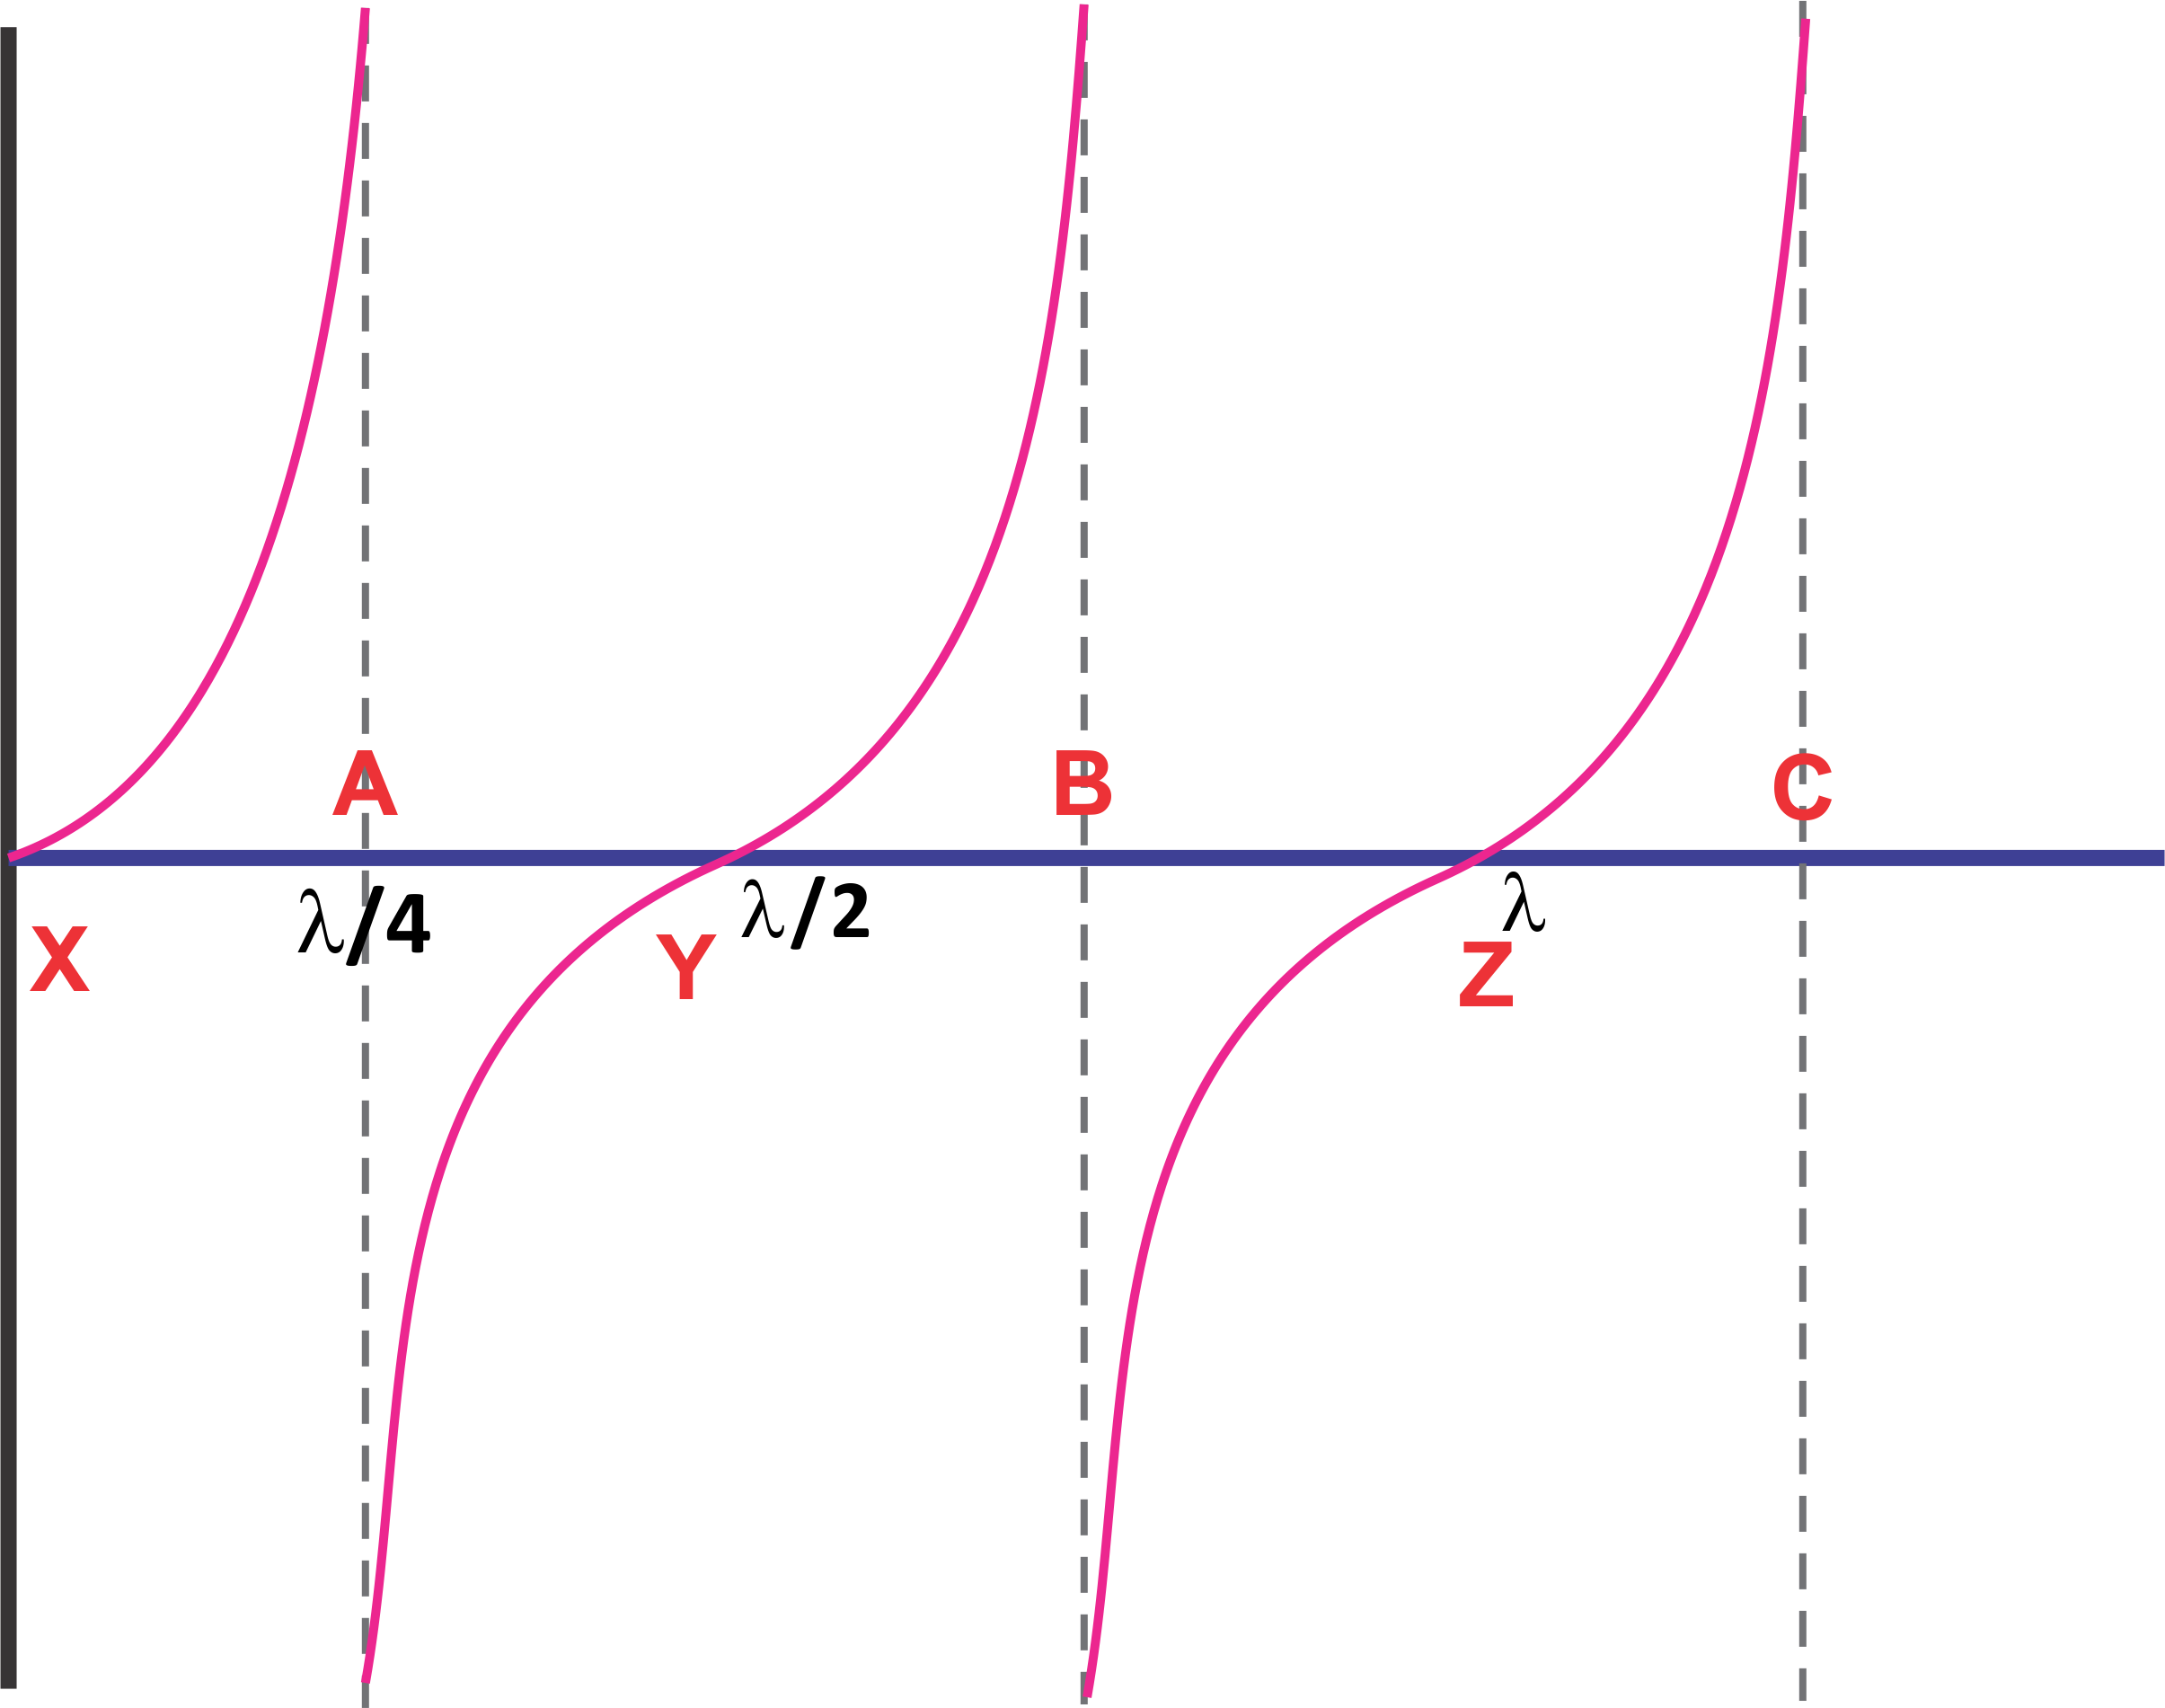
\includegraphics[scale=0.5]{./graphics/group10diagram10}
\caption{Short Circuit Line impedance change with frequency}
\end{figure}

For a short circuit whose length is $ \frac{\lambda}{2} $,(because it is repeating itself) the impedance is equal to zero. At $ \frac{\lambda}{4} $ the line will be an open circuit and the impedance will be $\infty$. One side of that frequency will be capacitive i.e negative. So when  the frequency is such that the length is zero(0) or $ \frac{\lambda}{2} $ or $ \lambda $ we get zero impedance.\\

However, if we go to the frequency for which the length is $ \frac{\lambda}{4} $, the impedance seen between the terminals of the lines is $\infty$ since it will appear like an open circuit.
So for a given frequency as we change the line length, when the line length is 0, $ \frac{\lambda}{2} $,$ \lambda $ we see impedances at X, Y and Z. At frequency for which the length is $ \frac{\lambda}{4} $, $ \frac{3\lambda}{4} $, $ \frac{5\lambda}{4} $ we are at A, B and C.\\ 
\textbf{NOTE:} We are dealing with short circuit for this example. Starting from short circuit (SC) point on Smith chart $ \frac{\lambda}{4} $, $ \frac{3\lambda}{4} $, $ \frac{5\lambda}{4} $ movement will place you at open circuit or $ \infty $,  hence A, B and C on the graph. $ \frac{\lambda}{2} $, $ \lambda $, $ \frac{3\lambda}{2} $ will place you back at the SC point where you  started from since a complete $ 2\pi $ movement correspond to $ \frac{\lambda}{2} $ on the Smith chart. Hence in the frequency range close to X,
Y and Z you have similar characteristics to a series LC circuit
at resonance.

However in the vicinity of A, B and C the behavior is similar to a parallel LC circuit at resonance. From the characteristics of series and parallel resonance circuits, we know that:
\begin{figure}[h]
\centering
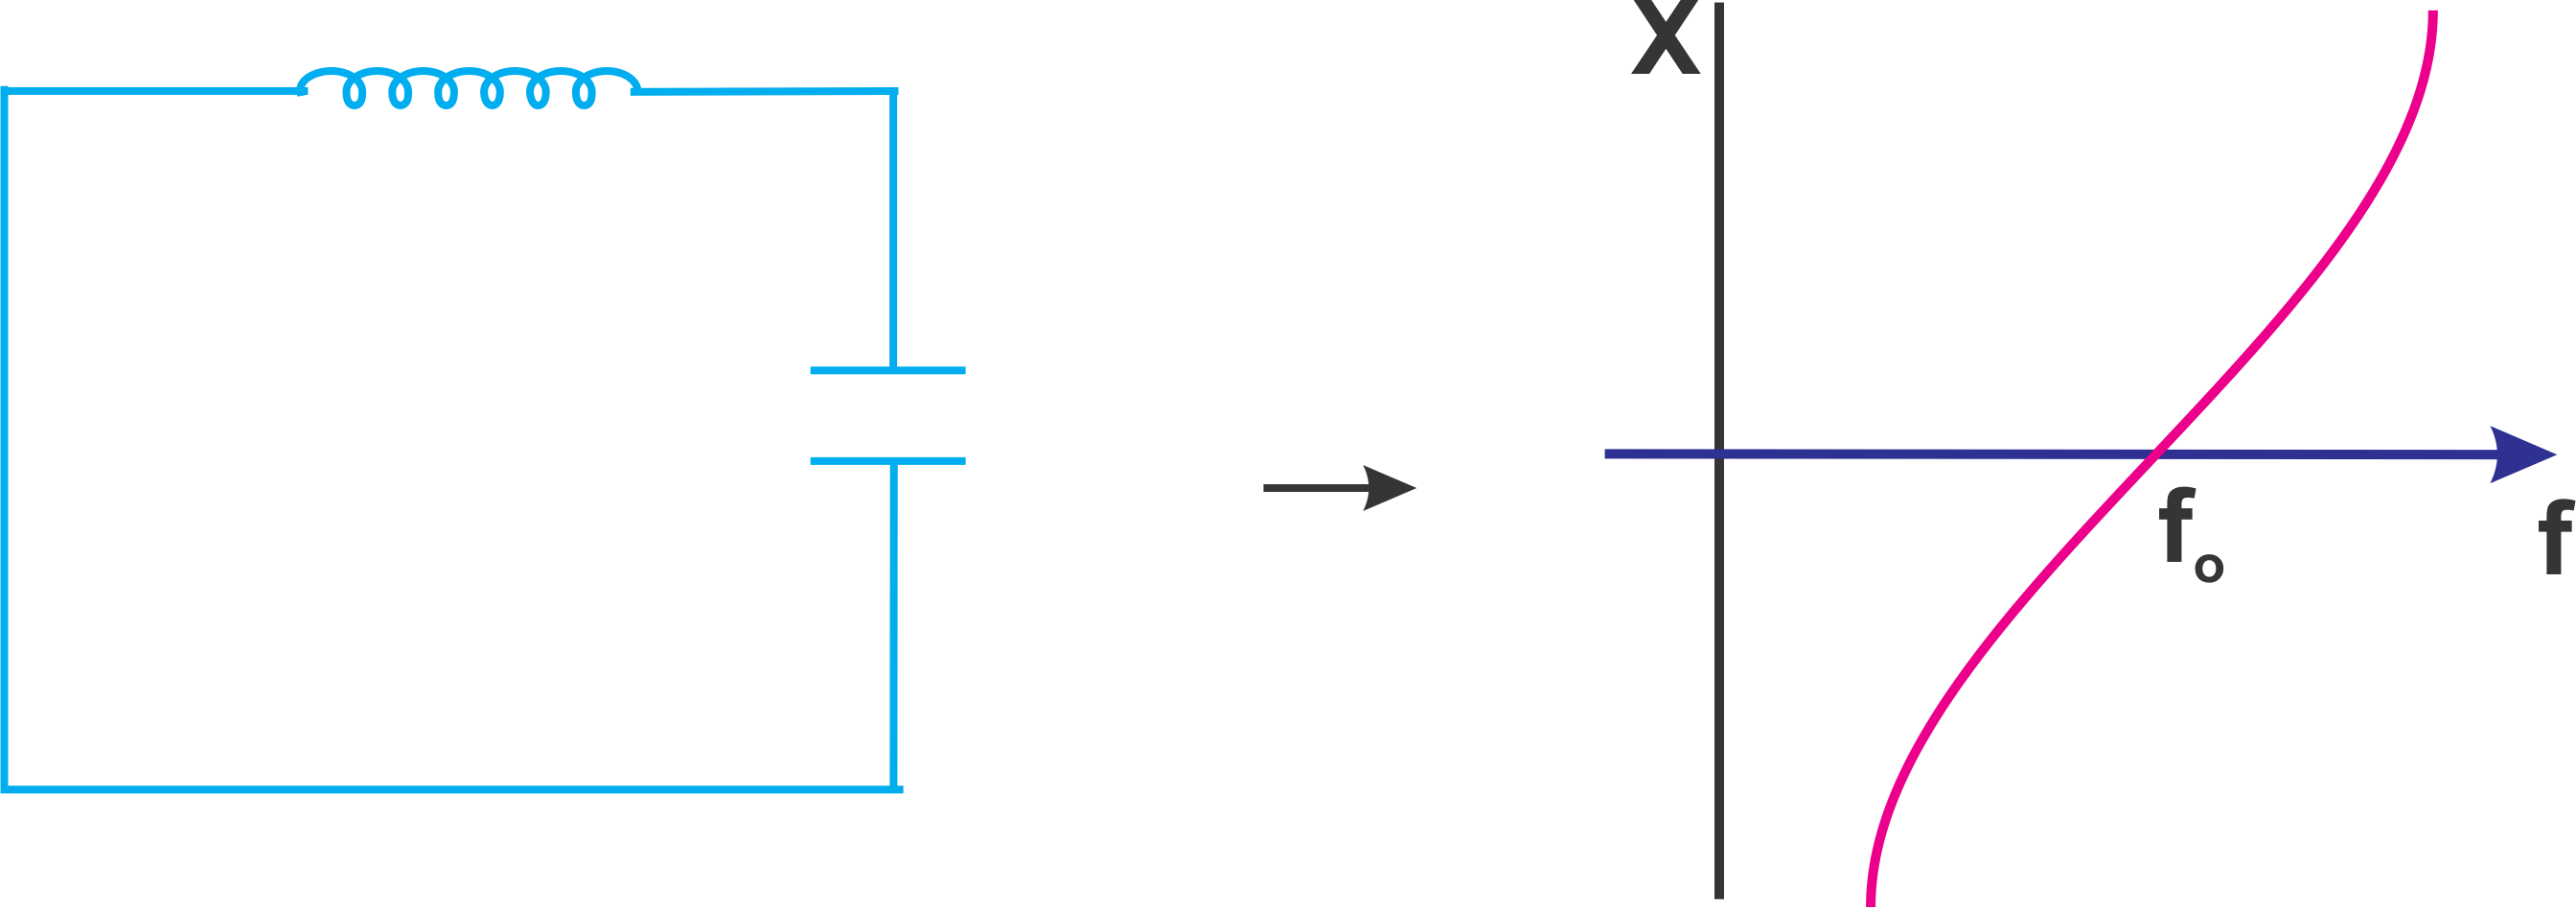
\includegraphics[width=1\linewidth]{./graphics/group10diagram11}
\caption{Series LC Circuit}
\end{figure}

(i) For Series LC Circuit, as you increase frequency $ X_{L} > X_{C} $ you have positive X, as you decrease frequency $ X_{C} > X_{L} $ you have negative X
\begin{figure}[h]
\centering
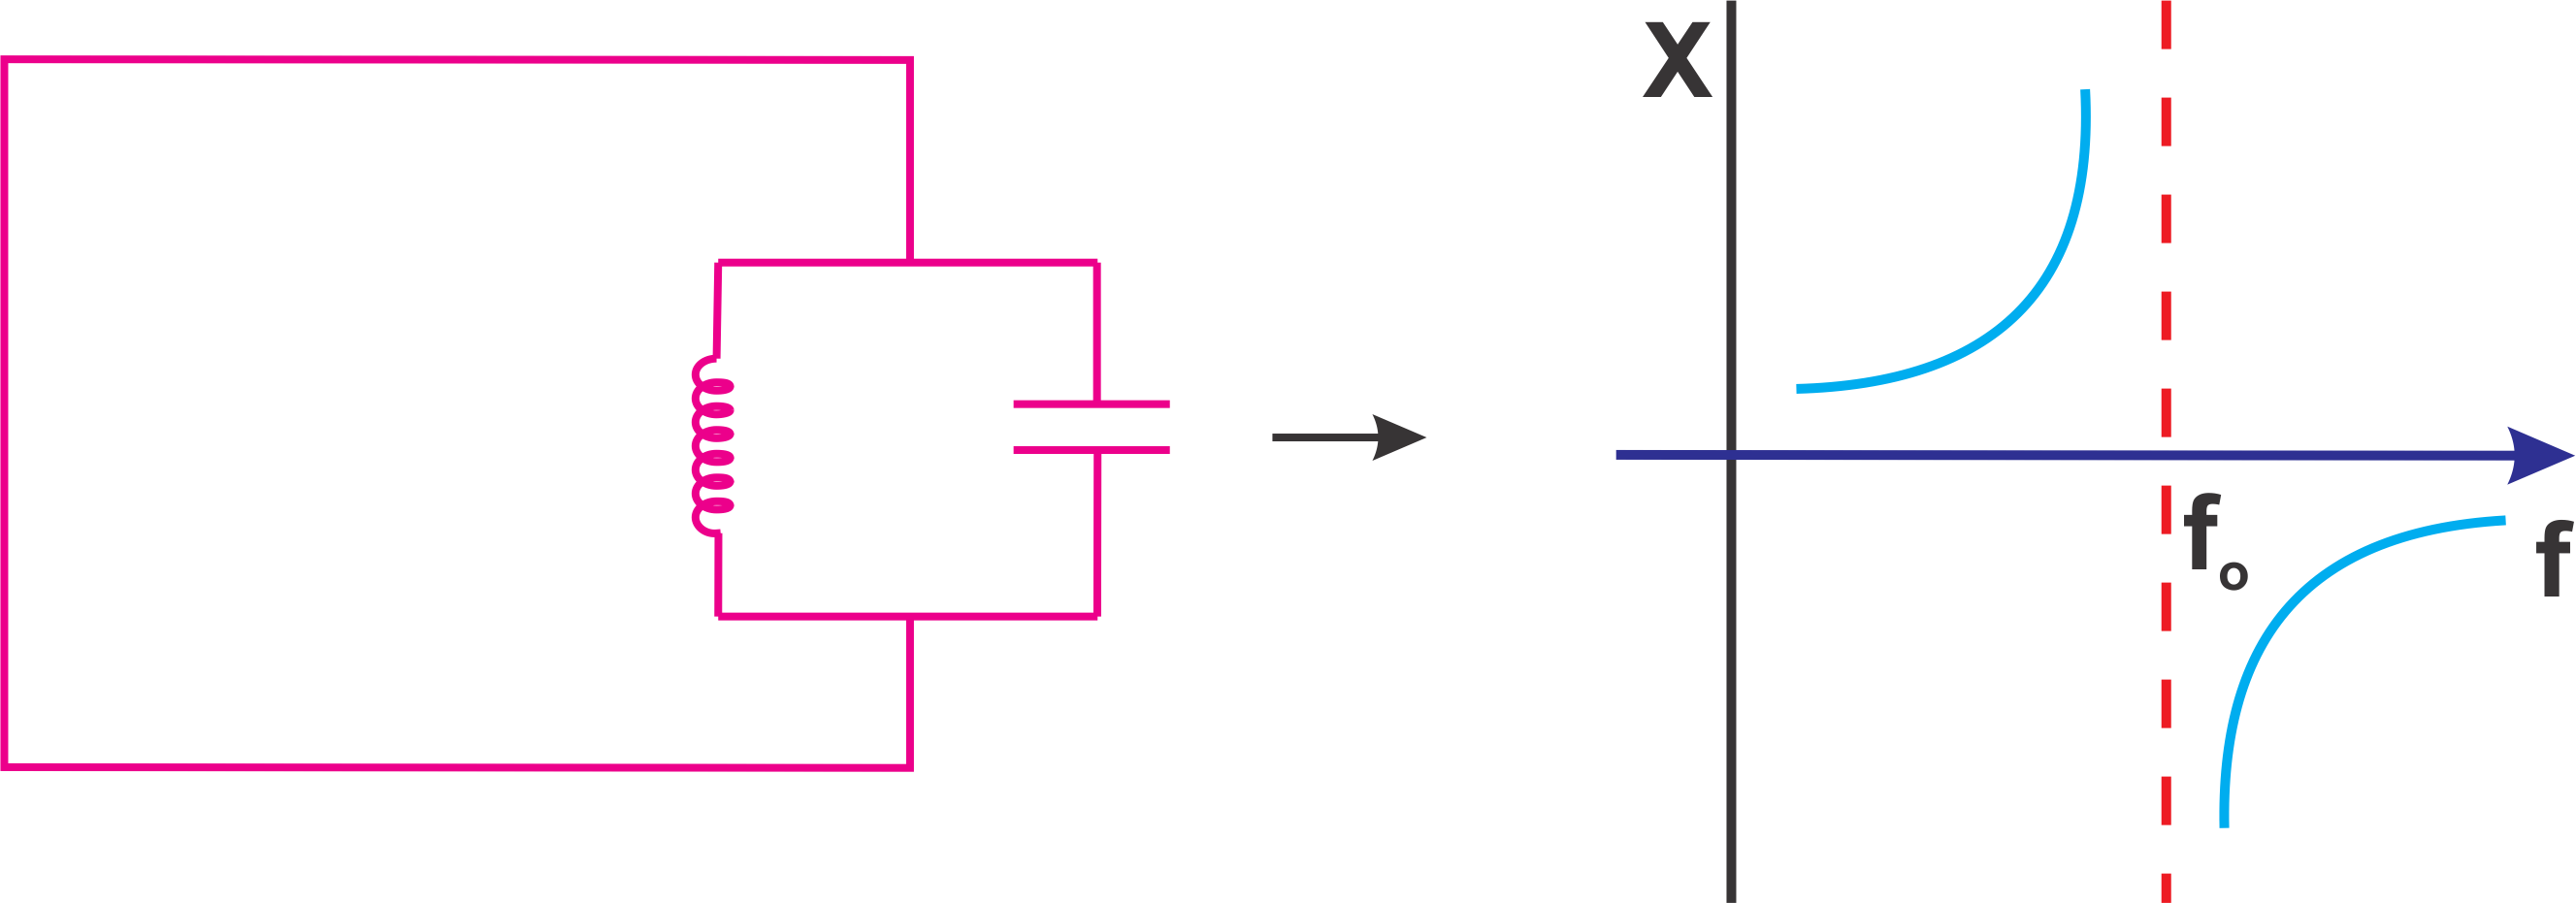
\includegraphics[width=1\linewidth]{./graphics/group10diagram12}
\caption{Parallel LC Circuit}
\end{figure}

(ii) At resonance frequency, X will become infinity. At lower frequency, $ X_{L} $ compared to $ X_{C} $, $ \frac{1}{X_{L}} $ is larger than $ \frac{1}{X_{C}} $. So $ X_{L} $ component dominates in the equivalent X. $ \frac{1}{X} = \frac{1}{X_{C}} + \frac{1}{X_{L}}$
\begin{align*}
\frac{1}{X_{C}} + \frac{1}{X_{L}} = 0\\
-jX + jX = 0 (X_{L} = X_{C})\\
\frac{1}{X} = 0, X = \frac{1}{0} = \infty
\end{align*}

So a line can behave like a series resonance circuit  if the frequency characteristics is like that of a series LC circuit, and can behave like an open circuit when behavior is like that of parallel LC circuits.
For a given length of transmission line, those frequencies for which the length of the line is close to $ \frac{\lambda}{2} $ the line will behave like series resonance circuit. On the other hand for those frequencies for which the length of the line is close to $ \frac{\lambda}{4} $, the line behaves like a parallel resonance circuit.\\
\textbf{NOTE:} The above explanation is for a SHORT circuited line while the exact OPPOSITE is for an OPEN circuited line.\\

For an open circuit whose length is $ \frac{\lambda}{2} $, the impedance is equal to infinity. At $ \frac{\lambda}{4} $ the line will be a short circuit and the impedance will be equal to zero. One side of that frequency will be capacitive i.e negative. So when the frequency is such that the length is zero(0) or $ \frac{\lambda}{2} $ or $ \lambda$ we get an impedance equal to infinity.
\begin{figure}[h]
\centering
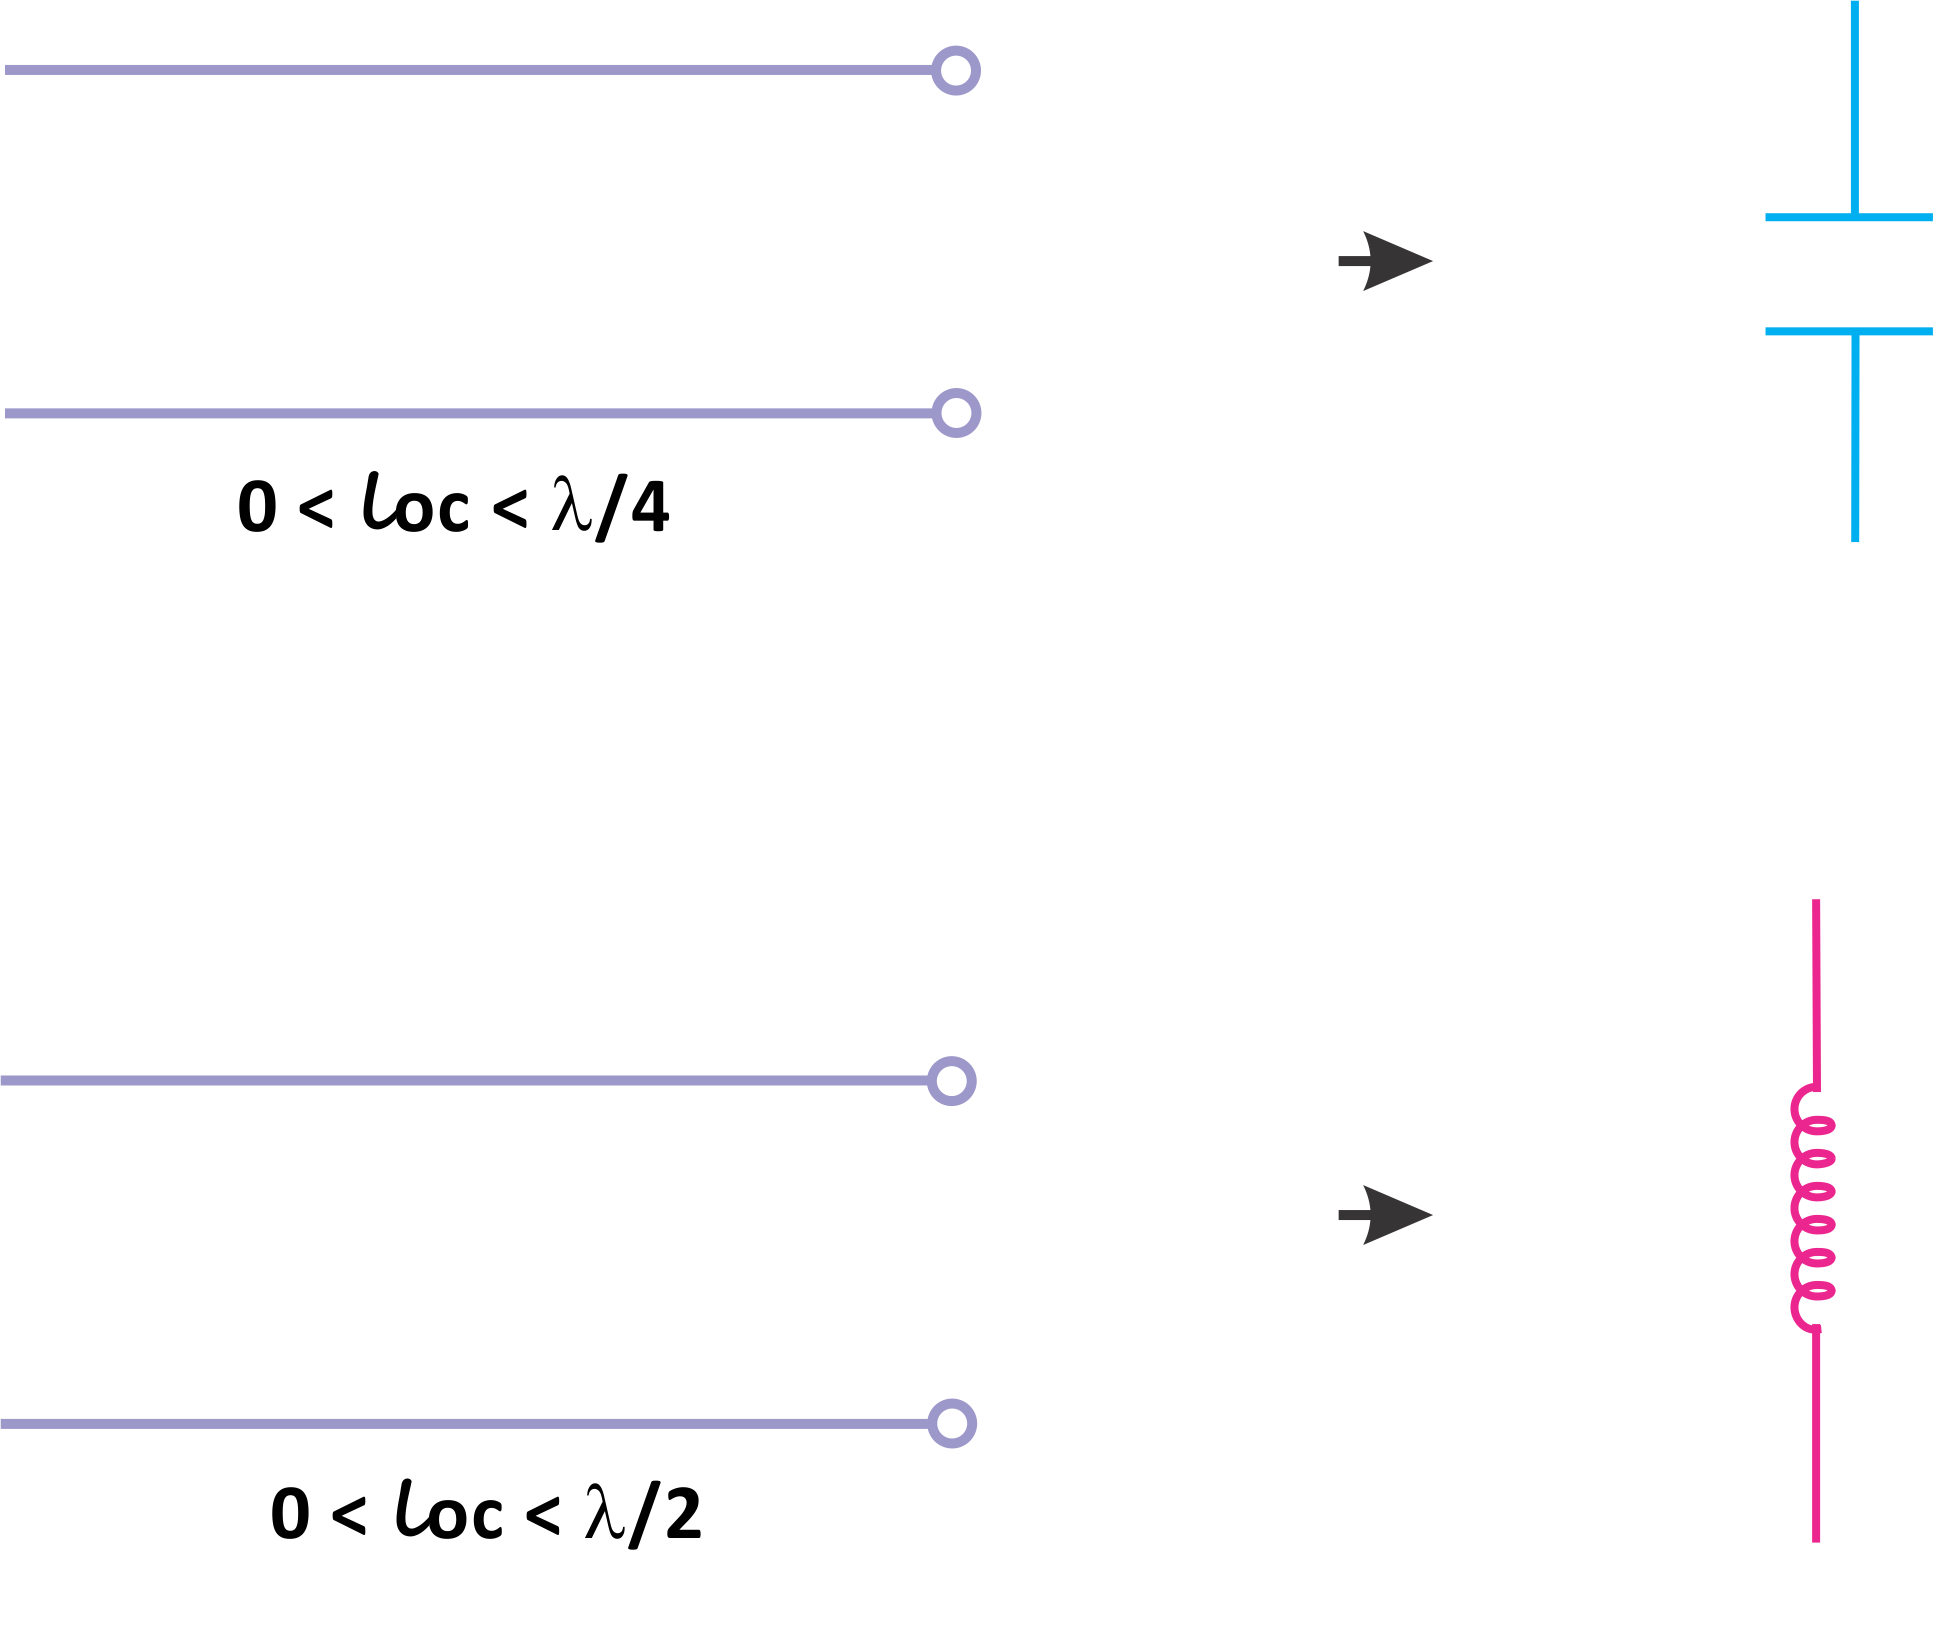
\includegraphics[scale=0.4]{./graphics/group10diagram13}
\end{figure}\\However, if we go to the frequency for which the length is $ \frac{\lambda}{4} $ , the impedance seen between the terminals of the lines is zero, since it will appear like a short circuit. So for a given frequency as we change the line length, when the line
length is 0, $ \frac{\lambda}{2} $ ,$ \lambda $ we see impedances at A, B and C. At frequency for which the length is $ \frac{\lambda}{4} $ , $ \frac{3\lambda}{4} $ , $ \frac{5\lambda}{4} $ we are at X, Y and Z.
\begin{figure}[h]
\centering
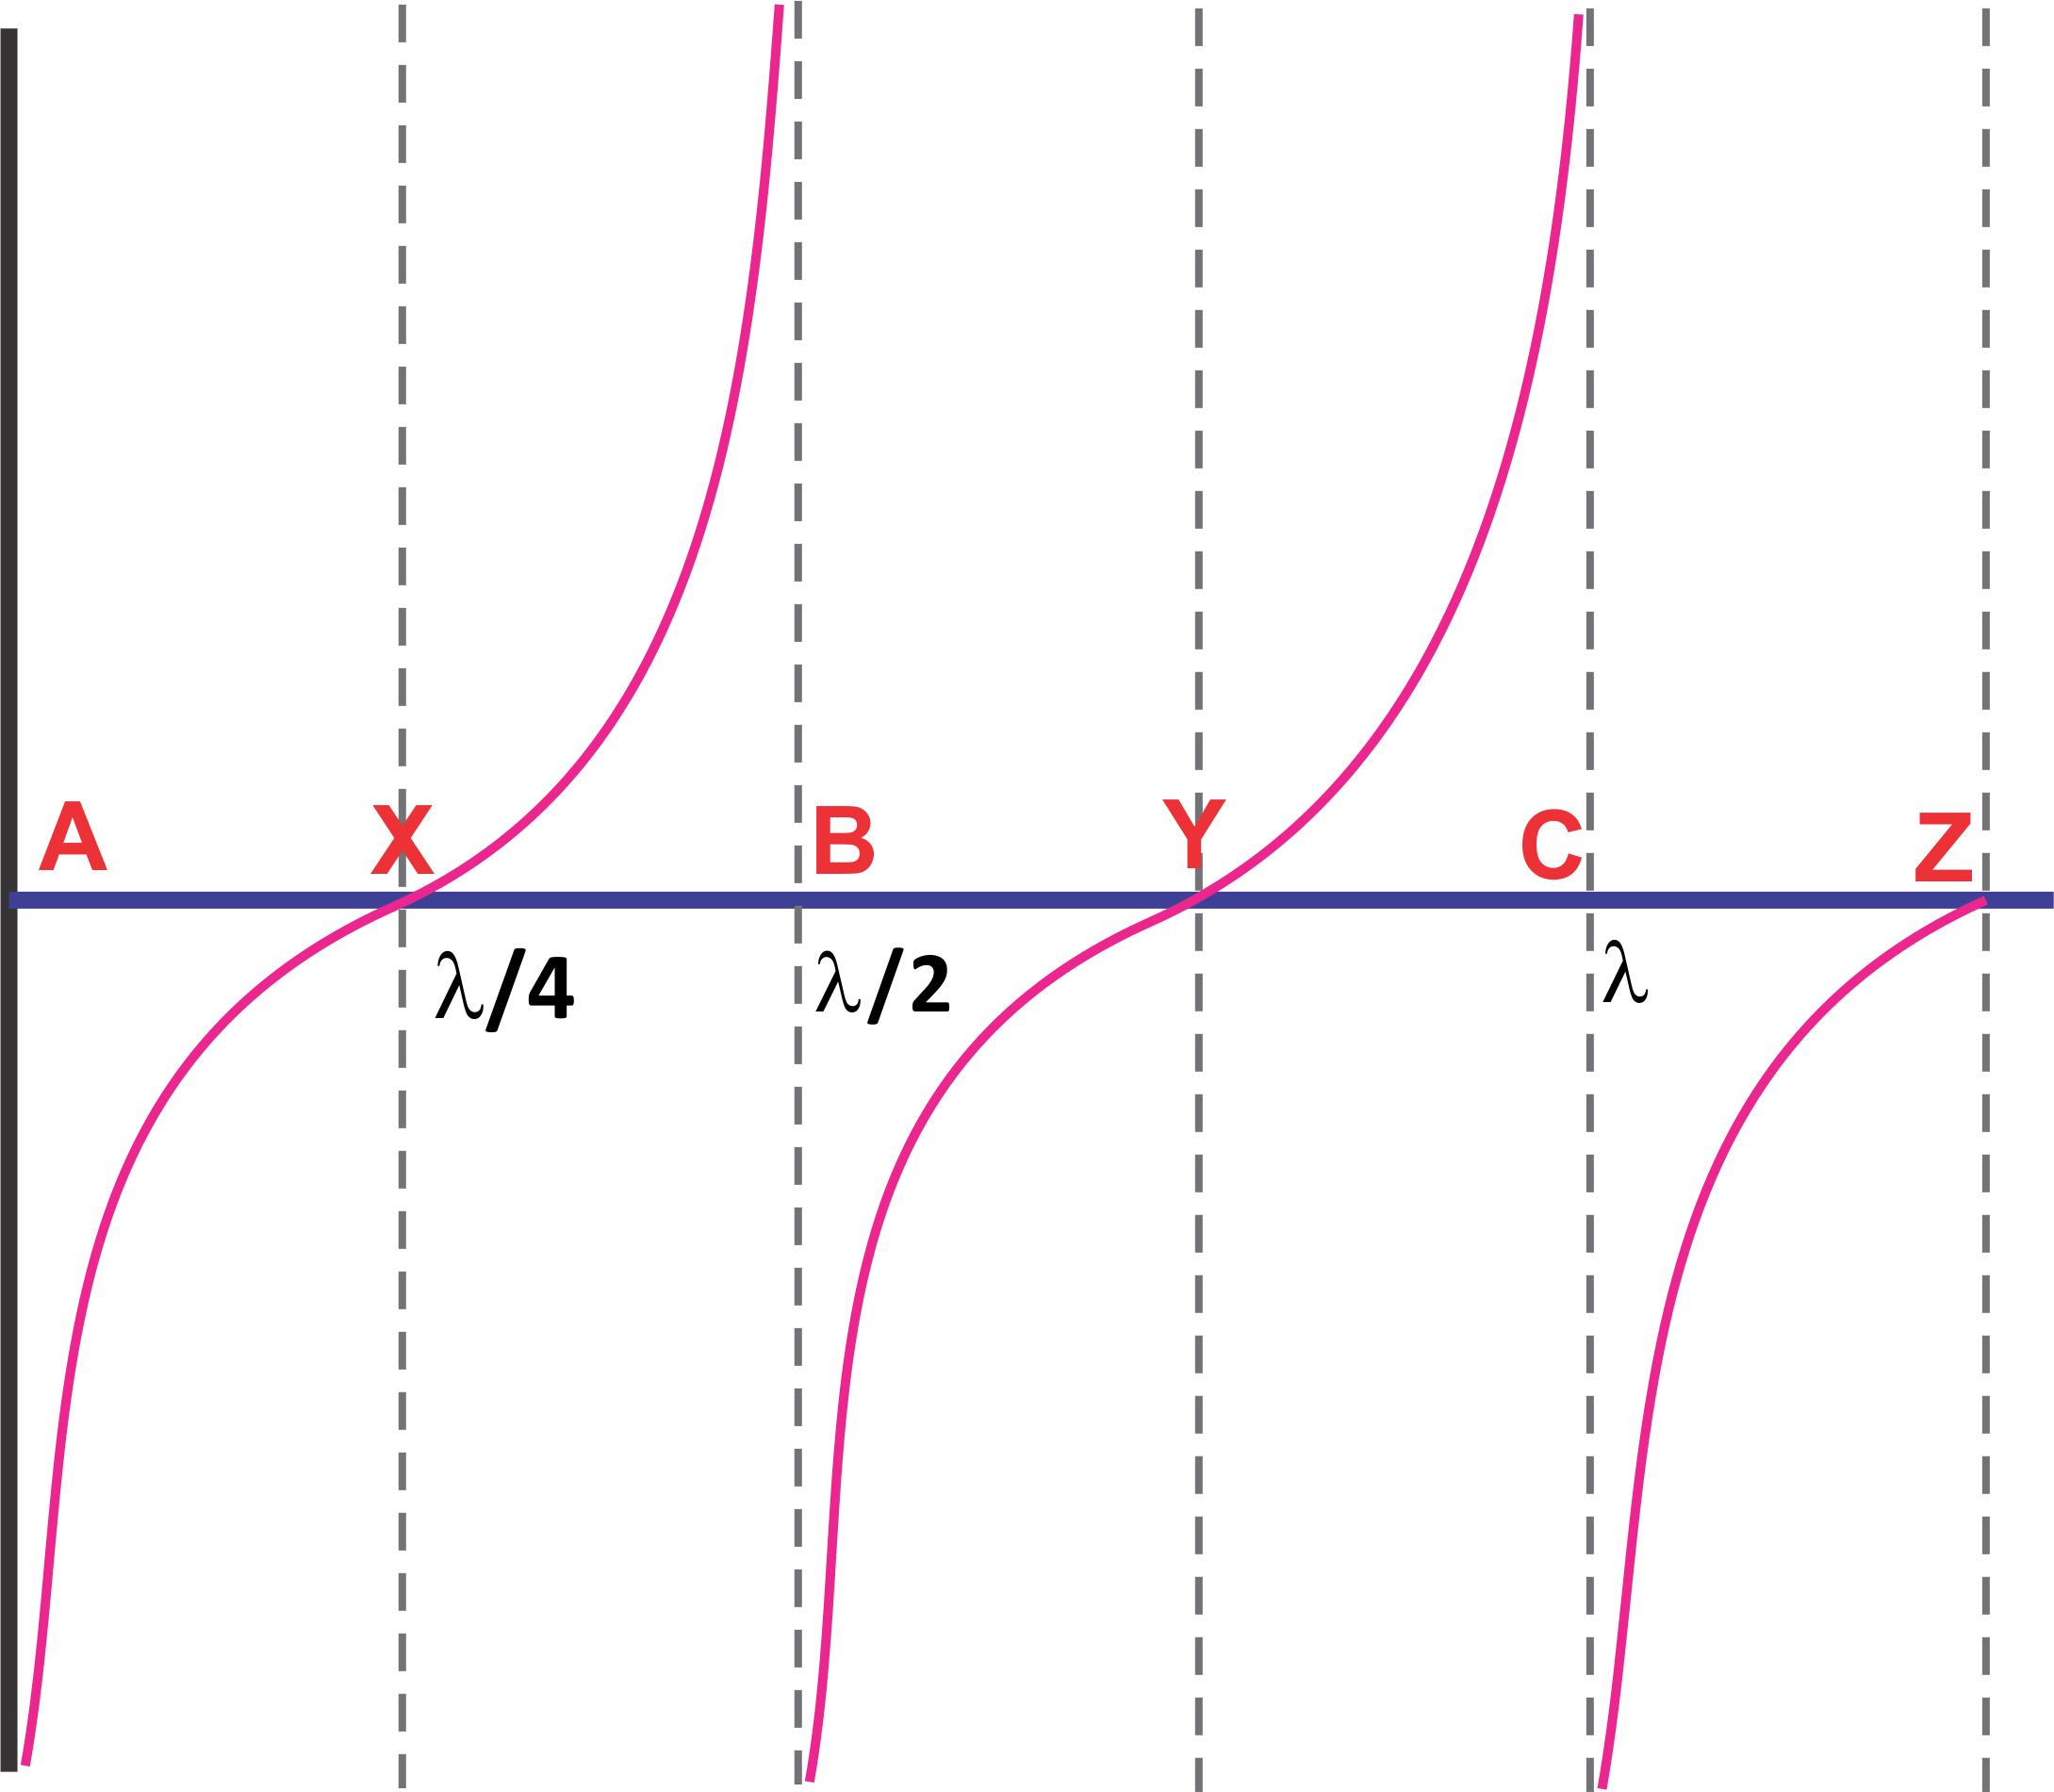
\includegraphics[scale=0.4]{./graphics/group10diagram14}
\caption{Open Circuit Line impedance change with frequency}
\end{figure}\\For open circuit line for length around $ \frac{\lambda}{2} $, the line will behave like a parallel resonant circuit because the input impedance will be at infinity. At about $ \frac{\lambda}{4} $, the line is like a short circuit and so behaves like a series resonant circuit. If the length of the line is $ \frac{\lambda}{2} $ the line will behave like a parallel resonant circuit.
So depending upon whether short circuit line or open circuit line is used, the series or parallel resonance circuit can be realized at different frequencies. So invariably, when we go to high frequencies, the line can be realized for getting reactive elements into the circuits. The line can also be used for realizing series or parallel resonance circuit into high frequency circuits.\\
So what is the quality factor of the resonant circuit?

By definition, quality factor is related to the losses of the circuit (The higher the loss, the smaller the quality factor). So whenever we have a reactive element like inductor or capacitor, the losses in these elements characterize the quality factor\footnote{Quality Factor is a parameter that describes how under-damped an oscillator or resonator is and characterizes a resonator's bandwidth relative to its center frequency. It is a dimensionless quantity.
It is a measure of the quality of a resonant circuit}. Since we are dealing with this transmission line as a lossless transmission line, the quality factor for these resonance circuits is infinite.\\
There is no loss, however in practice, there is always a small loss in the transmission line. Up till now we have treated the transmission line as lossless transmission line, because we were not really interested in the small loss. However, if we treat the line as lossless line, the quality factor will always be infinity. When we are interested in finding the quality factor of the resonance circuit, no matter how small the loss of the transmission
Line may be, we have to include the loss of the transmission line and then calculate the quality factor.
